\documentclass[a4paper,12pt]{report}
\raggedbottom
% polyglossia should go first!
\usepackage{polyglossia} % multi-language support

\setdefaultlanguage{russian}
\setmainfont{CMU Serif}
\setsansfont{CMU Sans Serif}
\setmonofont{CMU Typewriter Text}

\setmainlanguage{russian}
\setotherlanguage{english}

\DeclareSymbolFont{letters}{\encodingdefault}{\rmdefault}{m}{it}
\usepackage{amsmath} % math symbols, new environments and stuff
%\usepackage{bm}
\usepackage{unicode-math} % for changing math font and unicode symbols
\usepackage{identfirst}
\setmathfont{XITS Math}

\parindent=1.5cm
\usepackage{indentfirst}
\usepackage[left=2cm,right=1cm,top=2cm,bottom=2cm,bindingoffset=1cm]{geometry}% 
%for margins in title page
\renewcommand{\baselinestretch}{1.5}

\usepackage[style=english]{csquotes} % fancy quoting
\usepackage{microtype} % for better font rendering
\usepackage[backend=biber, sorting=none, style=gost-numeric]{biblatex} % for 
%bibliography
\addbibresource{reference_list.bib}

\usepackage{hyperref} % for refs and URLs
\usepackage{graphicx} % for images (and title page)
\usepackage{tabu} % for tabulars (and title page)
\usepackage{placeins} % for float barriers
\usepackage{titlesec} % for section break hooks

\usepackage[labelsep=endash]{caption}
\captionsetup[table]{
    singlelinecheck=false, %table caption per GOST, not centered
    justification=justified}
\captionsetup[figure]{
    name=Рисунок           %picture caption per GOST
}

\usepackage{subcaption} % for subfloats

\usepackage{listings} % for listings
\newfontfamily\listingsfont{Source Code Pro}

\usepackage{enumitem} % for unboxed description labels (long ones)
\usepackage{tikz}     % tikz pictures
\usepackage{rotating} % landscape pictures

\defaultfontfeatures{Mapping=tex-text} % for converting "--" and "---"

\MakeOuterQuote{"} % enable auto-quotation

% new page and barrier after section, also phantom section after clearpage for
% hyperref to get right page.
% clearpage also outputs all active floats:
\newcommand{\sectionbreak}{\clearpage\phantomsection}
\newcommand{\subsectionbreak}{\FloatBarrier}
\newcommand\numberthis{\addtocounter{equation}{1}\tag{\theequation}}
\renewcommand{\thesection}{\arabic{section}} % no chapters
\numberwithin{equation}{section}

\setcounter{tocdepth}{3}

\usepackage{lastpage}
\usepackage[figure,table,xspace]{totalcount}

\usepackage{array}
\newcolumntype{L}[1]{>{\raggedright\let\newline\\\arraybackslash\hspace{0pt}}m{#1}}
\newcolumntype{C}[1]{>{\centering\let\newline\\\arraybackslash\hspace{0pt}}m{#1}}
\newcolumntype{R}[1]{>{\raggedleft\let\newline\\\arraybackslash\hspace{0pt}}m{#1}}

\makeatletter
\define@key{blx@lbx}{fromjapanese}{\blx@defstring{fromjapanese}{#1}}
\define@key{blx@lbx}{langjapanese}{\blx@defstring{langjapanese}{#1}}
\makeatother

%algorithm2e
\usepackage{algorithm2e}
\SetKwInput{KwData}{Исходные параметры}
\SetKwInput{KwResult}{Результат}
\SetKwInput{KwIn}{Входные данные}
\SetKwInput{KwOut}{Выходные данные}
\SetKwIF{If}{ElseIf}{Else}{если}{тогда}{иначе если}{иначе}{конец условия}
\SetKwFor{While}{до тех пор, пока}{выполнять}{конец цикла}
\SetKw{KwTo}{от}
\SetKw{KwRet}{возвратить}
\SetKw{Return}{возвратить}
\SetKwBlock{Begin}{начало блока}{конец блока}
\SetKwSwitch{Switch}{Case}{Other}{Проверить значение}{и выполнить}{вариант}{в противном случае}{конец варианта}{конец проверки значений}
\SetKwFor{For}{цикл}{выполнять}{конец цикла}
\SetKwFor{ForEach}{для каждого}{выполнять}{конец цикла}
\SetKwRepeat{Repeat}{повторять}{до тех пор, пока}
\SetAlgorithmName{Рисунок}{рисунок}{Список алгоритмов}


\def\bm#1{\textbf{\textit{#1}}}
\def\dd#1{\frac{\p}{#1}}
\def\half{\frac{1}{2}}
\def\quart{\frac{1}{4}}
\def\dd#1{\frac{\p}{#1}}
\def\vvec{\ensuremath{\bm{v}}}
\def\vsq{\ensuremath{\vvec^2}}
\def\vr{\ensuremath{v_r}}
\def\vp{\ensuremath{v_\varphi}}
\def\p{\ensuremath{\partial}}
\DeclareMathOperator{\sizeof}{sizeof}

%\spvek{a;b;c;d} -> vector column
\makeatletter
\newcommand{\spvek}[2][r]{%
    \gdef\@VORNE{1}
    \left(\hskip-\arraycolsep%
    \begin{array}{#1}\vekSp@lten{#2}\end{array}%
    \hskip-\arraycolsep\right)}

\def\vekSp@lten#1{\xvekSp@lten#1;vekL@stLine;}
\def\vekL@stLine{vekL@stLine}
\def\xvekSp@lten#1;{\def\temp{#1}%
    \ifx\temp\vekL@stLine
    \else
    \ifnum\@VORNE=1\gdef\@VORNE{0}
    \else\@arraycr\fi%
    #1%
    \expandafter\xvekSp@lten
    \fi}
\makeatother


\begin{document}
%skip for title page
\textbf{\large{Реферат}}.

Отчёт \pageref{LastPage}с., \totalfigures рис., \totaltables табл., 
TODO источников.

\noindent \textbf{ Локализация, Построение карты местности, Одновременная локазизация и построение карты местности, SLAM, Многоагентная SLAM }

Работа направлена на создание ПО для решения задачи одновременной локализации и построения трехмерной карты местности множеством агентов, оснащенных одной RGB камерой.

Цель проекта - создание алгоритмов и программно-математического 
обеспечения для моделирования тепло- и электрофизических процессов, описываемых 
системами многомерных нелинейных уравнений в частных производных и обыкновенных 
дифференциальных уравнений, а также исследование применимости разработанного ПО 
для решения различных научных задач.

Предложен общий подход к решению систем разнородных 
уравнений и выделены основные типы математических подзадач, 
проведен анализ методов решения и выполнена их реализация. Разработана 
структура ПО и структуры хранения данных. Создан набор приложений для 
формирования исходных данных моделей, решения соответствующих уравнений и 
визуализации полученных 
результатов. Приведены примеры использования разработанного ПО в вычислительных 
экспериментах, в том числе включающих расчёт средствами платформы CUDA. 
Результаты численного моделирования сравниваются с данными натурного 
эксперимента.
Показана работоспособность ПО при проведении прикладных исследований.

\setcounter{page}{5}
\tableofcontents

\section{Введение}
В данной работе идет речь о построении трехмерной карты местности множеством агентов, на основе некоторой информации об окружении, получаемой ими независимо друг от друга. Эта задача имеет множество
вариантов решения, в зависимости от вычислительной мощности агентов, их оснащения для получения информации об окружающей среде и допустимых энергетических затратах агентов на передвижение. Также, вариант решения задачи может максимизировать точность построения карты и ее качество или делать упор на максимизацию скорости определения местоположения в пространстве. Все эти факторы определяют требования к методу
решения задачи SLAM, набор алгоритмов, необходимых для локализации в пространтстве на основе набора извлеченных некоторым образом его характеристик, формат представления карты и набор алгоритмов построения карты. Наименее исследованной областью является построение трехмерной карты местности в режиме реального времени с аппаратными требованиями к агенту на уровне доступной любительской техники~\cite{SLAMoverview}


Актуальность выбранной темы обусловлена набором задач, автоматизация которых возможна при помощи одного или нескольких беспилотных наземных или летательных аппаратов, например:
\begin{itemize}
    \item решение сложных задач группового взаимодействия, при котором агентам необходимо иметь информацию о положении друг относительно друга (логистические задачи доставки определенных грузов или предметов без привязки к априорно изветной карте местности, где выгоду приносит возможность передачи предметов между агентами)~\cite{beerSLAM};
    \item навигация беспилотных наземных транспортных средств, где построение карты местности позволяет обновлять информацию о текущей дорожной ситуации~\cite{kittyDataset};
    \item построение карты местности объектов с затрудненным доступом для человека, вследствие природных, техногенных и иных факторов~\cite{tum3DMonoSLAM};
    \item построение трехмерных карт объектов исторической и культурной ценности.
\end{itemize}
Возрастающие аппаратные возможности простых беспилотных летательных аппаратов, таких как квадрокоптеры, обуславливает тенденцию роста~\cite{tum3DMonoSLAM} популярности темы данной работы.


Целью работы является разработка нового метода одновременной локализации и построения карты местности, сочетающего в себе ряд следующих характеристик:
\begin{itemize}
    \item локализация и построение карты местности производятся в реальном или близком к реальному времени (20 -- 60 кадров в секунду);
    \item метод обеспечивает построение трехмерной карты местности;
    \item метод предъявляет низкие(соответствующие современным квадрокоптерам) требования к аппаратному обеспечению и вычислительной мощности беспилотного аппарата, являющегося агентом;
    \item метод не требует специализированных устройств(таких как лидары, дальномеры) для получения информации об окружающей среде - допускается использование обычной поративной RGB камеры.
\end{itemize}
 

Для достижения посталенной цели необходимо решить следующие задачи:
\begin{itemize}
    \item извлечение информации о удаленности и масштабе объектов окружения агента;
    \item определение собственной скорости движения агентом на основе извлеченных данных об окружении;
    \item локализация в пространстве на основе извлеченной информации о расстоянии до объектов окружения и скорости передвижения;
    \item построение трехмерной карты местности на основе извлеченных данных о расстояниях до предметов окружения и локализации;
    \item разработка ПО для демонстрации и тестирования данного метода с использованием публично доступных наборов данных.
\end{itemize}

\section{Аналитический раздел}
\subsection{Введение}
В данном разделе приводится краткий обзор существующих методов решения SLAM. Производится сравнительный анализ алгоритмов, решающих поставленные задачи, делается вывод о обосновании выбора конкретных алгоритмов для решения поставленных задач.

\subsection{Локализация}
Существует два фундаментальных подхода к локализации:
\begin{itemize}
    \item формирование списка неподвижных опорных точек, извлеченных из окружения, и локализация на основе оценки положения опорных точек в каждый следующий момент времени;
    \item формирование списка ключевых кадров и локализация на основе вычисления аффинного преобразования от предыдущего кадра к последующему.
\end{itemize}


Первый подход используется в марковских методах~\cite{MDPSLAM} и методах, использующих фильтр Калмана~\cite{EKFSLAM}. Общий алгоритм локализации в таком случае состоит из двух операций: составления предположения о собсвенном местоположении в пространстве, на основе имеющихся данных о предыдущем местоположении и параметров движения, и уточнения оценки местоположения в пространстве, опираясь на новое измерение положения неподвижных опорных точек. Главным недостатком данных подходов является привязка к объектам окружения, которые в общем случае не являются неподвижными, что приводит к необходимости распознавания объектов окружения или введения механизма удаления опорных точек, что отражается на скорости работы алгоритма и его сходимости~\cite{EKFSLAM}. Также, ввиду того, что эти методы хранят информацию только о опорных точках, принципиально невозможно их использование для выполнения задачи построения карты местности.


Второй подход наиболее полно отвечает поставленной задаче, т.к. побочная информация этапа локализации может быть непосредственно использована для решения задачи построения карты местности. Алгоритм локализации по методу извлечения ключевых кадров сводится к вычислению аффинного преобразования текущего обозреваемого окружения к одному или нескольким имеющимся ключевым кадрам, положение в пространстве которых уже вычислено в процессе их извлечения, а положение первого ключевого кадра находится в начале координат. Локализация этим методом так же подразделяется на две фундаментально различные группы методов: извлекающие информацию из входного потока данных при помощи распознавания некоторых особенностей предметов, таких как наличие прямых или скругленных линий, и работающие напрямую со всей входной информацией без предварительного распознавания объектов окружения. Алгоритмы локализации на основе извлечения ключевых кадров с распознаванием объектов окружения являются более простыми с точки зрения реализации, поскольку для определения нового положения и параметров движения агента достаточно обработать только небольшую часть данных входного потока информации. Однако именно это преимущество определяет существенный недостаток - невозможность работы в окружениях, лишенных указанных при разработке алгоритма распознаваемых особенностей~\cite{tum3DMonoSLAM}. Таким образом, можно сделать вывод, что для реализации задачи локализации в трехмерном пространстве, сопряженной с последующим построением карты местности, следует использовать алгоритм локализации на основе ключевых кадров без распознавания особенностей окружения.


\subsection{Построение карты местности}
Формат представления карты и алгоритм ее построения являются сильно зависимыми от алгоритма локализации, т.к. побочным результатом выполнения задачи локализации является набор информации о положении объектов окружения. Исходя из того, что наиболее полно поставленной задаче локализации отвечает алгоритм на основе ключевых кадров, будут рассмотрены только алгоритмы построения карты местности, входными данными для которых является последовательность кадров окружения. В таком случае естественно следующим из структуры входных данных способом представления карты является неориентированный граф $G(K, E),$ где множество вершин $K$ -- это множество ключевых кадров, а множество дуг $E = K x K$ определяется последовательностью возникновения ключевых кадров во входной последовательности и обнаружением циклов в траектории движения агента.


Таким образом можно сделать вывод о том, что для решения задачи построения карты местности необходимо решить две поздазачи:
\begin{itemize}
    \item обновления карты при получении нового ключевого кадра,
    \item поиска циклов при добавлении нового ключевого кадра.
\end{itemize}


Конкретные алгоритмы решения этих подзадач определяются выбором математического аппарата представления положения агента в пространстве.


\subsection{Математический аппарат}
Существует множество подходов к представлению положения объекта в пространстве, каждый из которых является наиболее удобным для реализации алгоритма локализации. С учетом того, что локализация на основе ключевых кадров наиболее полно отвечает постановке задачи, необходим математический аппарат, способный успростить вычисление аффинных преобразований и упростить вычисление операций над этими преобразованиями, таких как композиция, вычисление обратного преобразования, вычисление якобиана и гессиана.


Из необходимости получения трехмерной карты следует, что все преобразования имею 7 степеней свободы - 3 вращательных, 3 поступательных и масштабирование. Эти операции могут быть обобщены с помощью двух математических аппаратов - использования кватернионов и использования групп Ли. В трехмерном пространтве все указанные аффинные преобразования задаются матрицей
\begin{equation}
    \begin{pmatrix}
    \mathbf{R} & \mathbf{t}  \\
    \mathbf{0} & \frac{1}{s} \\
    \end{pmatrix}
\end{equation}
,где $\mathbf{R}: 3x3$ -- матрица поворота, $\mathbf{t} \in \mathbb{R}^3$ -- вектор переноса, $s$ -- масштаб.


Наиболее полно предъявленным требованиям к математическому аппарату овечает алгебра Ли, оперирующая аффинными трансформациями в пространстве размерности равной числу степеней свободы($\mathbf{Sim3}$). Засчет введения дополнительных размерностей пространства, основные операции над матрицей преобразования могут быть существенно упрощены~\cite{lieGroups}:
\begin{itemize}
    \item композиция преобразований
    \begin{equation}
        \begin{pmatrix}
        \mathbf{R_1} & \mathbf{t_1}  \\
        \mathbf{0} & \frac{1}{s_1} \\
        \end{pmatrix}
        \cdot
        \begin{pmatrix}
        \mathbf{R_2} & \mathbf{t_2}  \\
        \mathbf{0} & \frac{1}{s_2} \\
        \end{pmatrix}
        =
        \begin{pmatrix}
        \mathbf{R_1}\mathbf{R_2} & \mathbf{R_1}\mathbf{t_2} + \frac{\mathbf{t_1}}{\mathbf{s_2}}  \\
        \mathbf{0} & \frac{1}{s_1 s_2} \\
        \end{pmatrix}, \mathbf{R_i} \in \mathbf{SO}(3), \mathbf{t} \in \mathbb{R}^3, s_i \in \mathbb{R}, i = \bar{1,2}
    \end{equation}
    \item вычисление обратной матрицы
    \begin{equation}
        \begin{pmatrix}
        \mathbf{R} & \mathbf{t}  \\
        \mathbf{0} & \frac{1}{s} \\
        \end{pmatrix}
        ^{\!\!-1}
        =
        \begin{pmatrix}
        \mathbf{R}^T & -s\mathbf{R}^T\mathbf{t} \\
        \mathbf{0} & s_1 \\
        \end{pmatrix}, \mathbf{R} \in \mathbf{SO}(3), \mathbf{t} \in \mathbb{R}^3, s \in \mathbb{R}
    \end{equation}
    \item вычисление якобиана существенно упрощается, засчёт упрощения дифференцирования по параметрам преобразования
    \begin{equation}
        \begin{align*}
            \mathbf{y} = \mathbf{R}\mathbf{x} \\
            \frac{\partial\mathbf{y}}{\partial\mathbf{R}}
            = -\mathbf{y} \cdot
            \begin{pmatrix}
            0 & -1 & 1 \\
            1 & 0 & -1 \\
            -1 & 1 & 0 \\
            \end{pmatrix}
        \end{align*}
    \end{equation}
\end{itemize}


Альтернативным математическим аппаратом для эффективной по времени работы с матрицами аффинных преобразований трехмерного евклидового пространства являются кватернионы, выполняющие эти преобразования в четырехмерном пространтве, однако вычисление якобиана при помощи этого аппарата является задачей, по времени выполнения сравнимой с классическим вычислением якобиана, что является недостатком этого математического аппарата, с точки зрения указанных требований. Таким образом, задача локализации будет выполняться в алгебре Ли $\textbf{Sim}(3)$

\subsection{Существующие аналоги}

\subsection{Общие принципы работы разрабатываемого ПО}


\subsection{Вывод}
Сформулированы общие принципы работы проектируемого ПО. Выбраны 
решаемые виды уравнений и выведены разностные схемы для решения 
дифференциальных уравнений в частных производных параболического и 
эллиптического типов. Приведен краткий обзор особенностей гиперболических 
уравнений и сделан вывод о нереализуемости достаточно общих методов их решения 
в рамках данной работы.

\section{Конструкторский раздел}
\subsection{Введение}
%942
В данном разделе приводятся соображения, касающиеся проектирования 
разрабатываемого ПО. Приводится описание структуры разработанного ПО и её 
формальное представление в виде диаграмм. Описываются разработанные структуры 
хранения данных, приводятся описания использованных алгоритмов.

\subsection{Структура ПО}
При проектировании данного ПО рассматривались следующие варианты его реализации:
\begin{itemize}
    \item Монолитный подход -- ПО представляет собой единую программу, 
    реализующую все требуемые функции от проведения моделирования до 
    визуализации результатов моделирования
    \item Модульный подход -- разделение ПО на несколько составных частей, 
    каждая из которых реализует определённую функцию
\end{itemize}
Использован был именно модульный подход, поскольку он позволяет как можно 
больше разделить ответственность между отдельными компонентами программы.

Таким образом, разрабатываемое ПО состоит из следующих частей:
\begin{itemize}
    \item Библиотека математических подпрограмм PDELib
    \item Утилита редактирования полей в полярных координатах (для задания 
    начальных распределений величин) PDEFieldCreator
    \item ПО для проведения вычислительного эксперимента PDESS
    \item Утилита визуализации результатов моделирования PDEVis
\end{itemize}

Утилиты PDEFieldCreator, PDESS и PDEVis зависимы от библиотеки PDELib.

Idef0-схема наиболее ресурсоёмкой утилиты, отвечающей за собственно расчёт 
модели, представлена на рисунке~\ref{fig:idef0-top}. Более подробно процесс 
проведения вычислительного эксперимента представлен на схемах на 
рисунке~\ref{fig:idef0-L1} и на рисунке~\ref{fig:idef0-L2}.

\begin{figure}
    \centering
    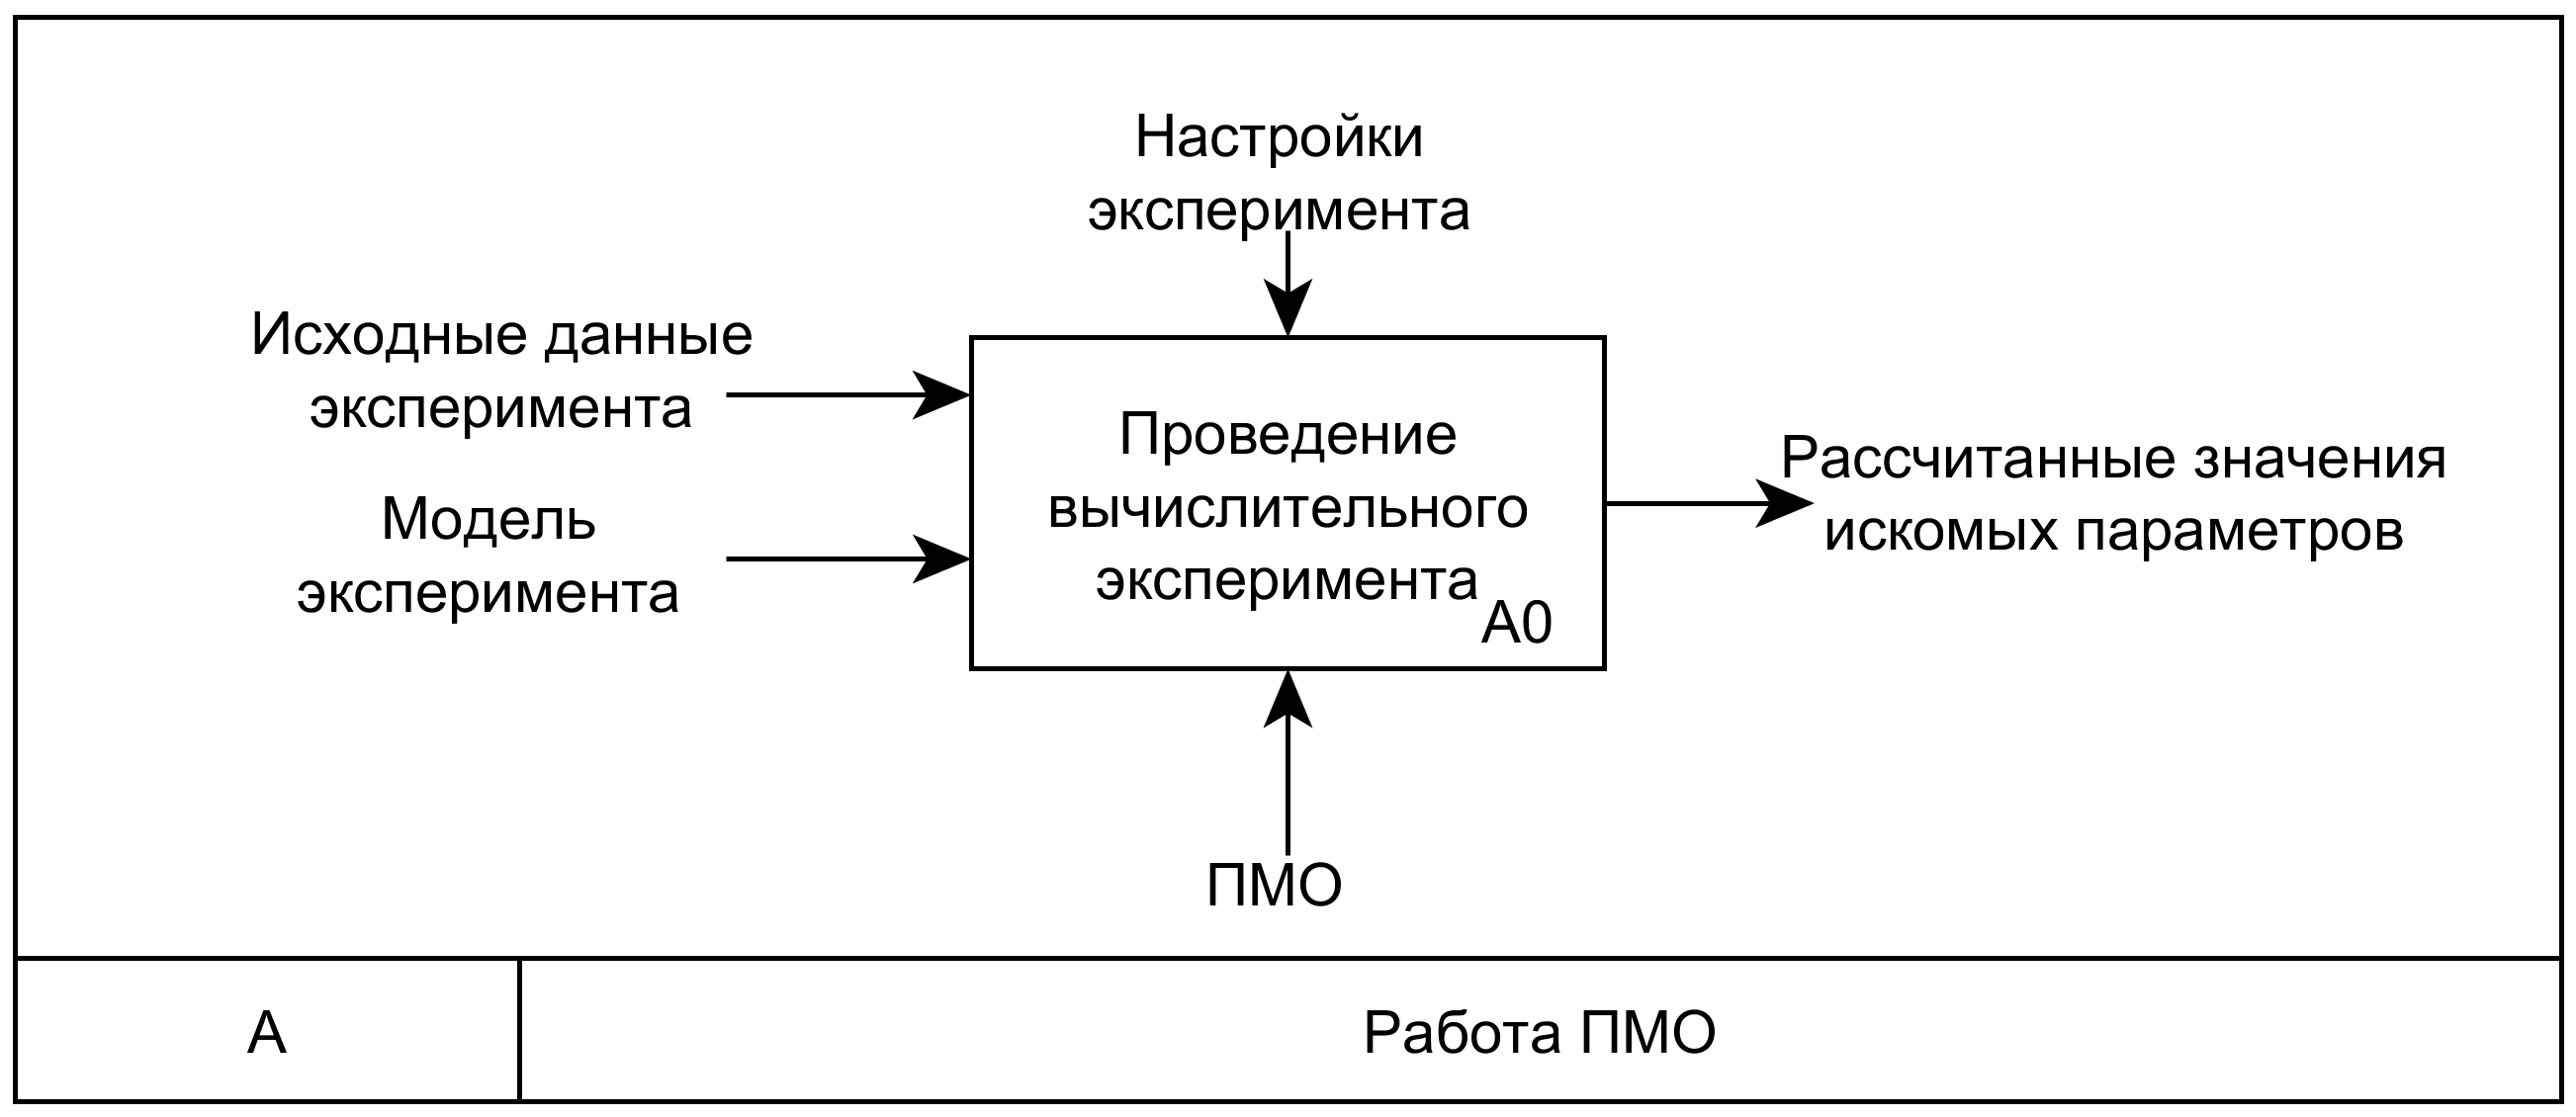
\includegraphics[width=.7\textwidth]{img/idef0/top}
    \caption{Idef0-диаграмма верхнего уровня утилиты расчёта модели}
    \label{fig:idef0-top}
\end{figure}

\begin{figure}
    \centering
    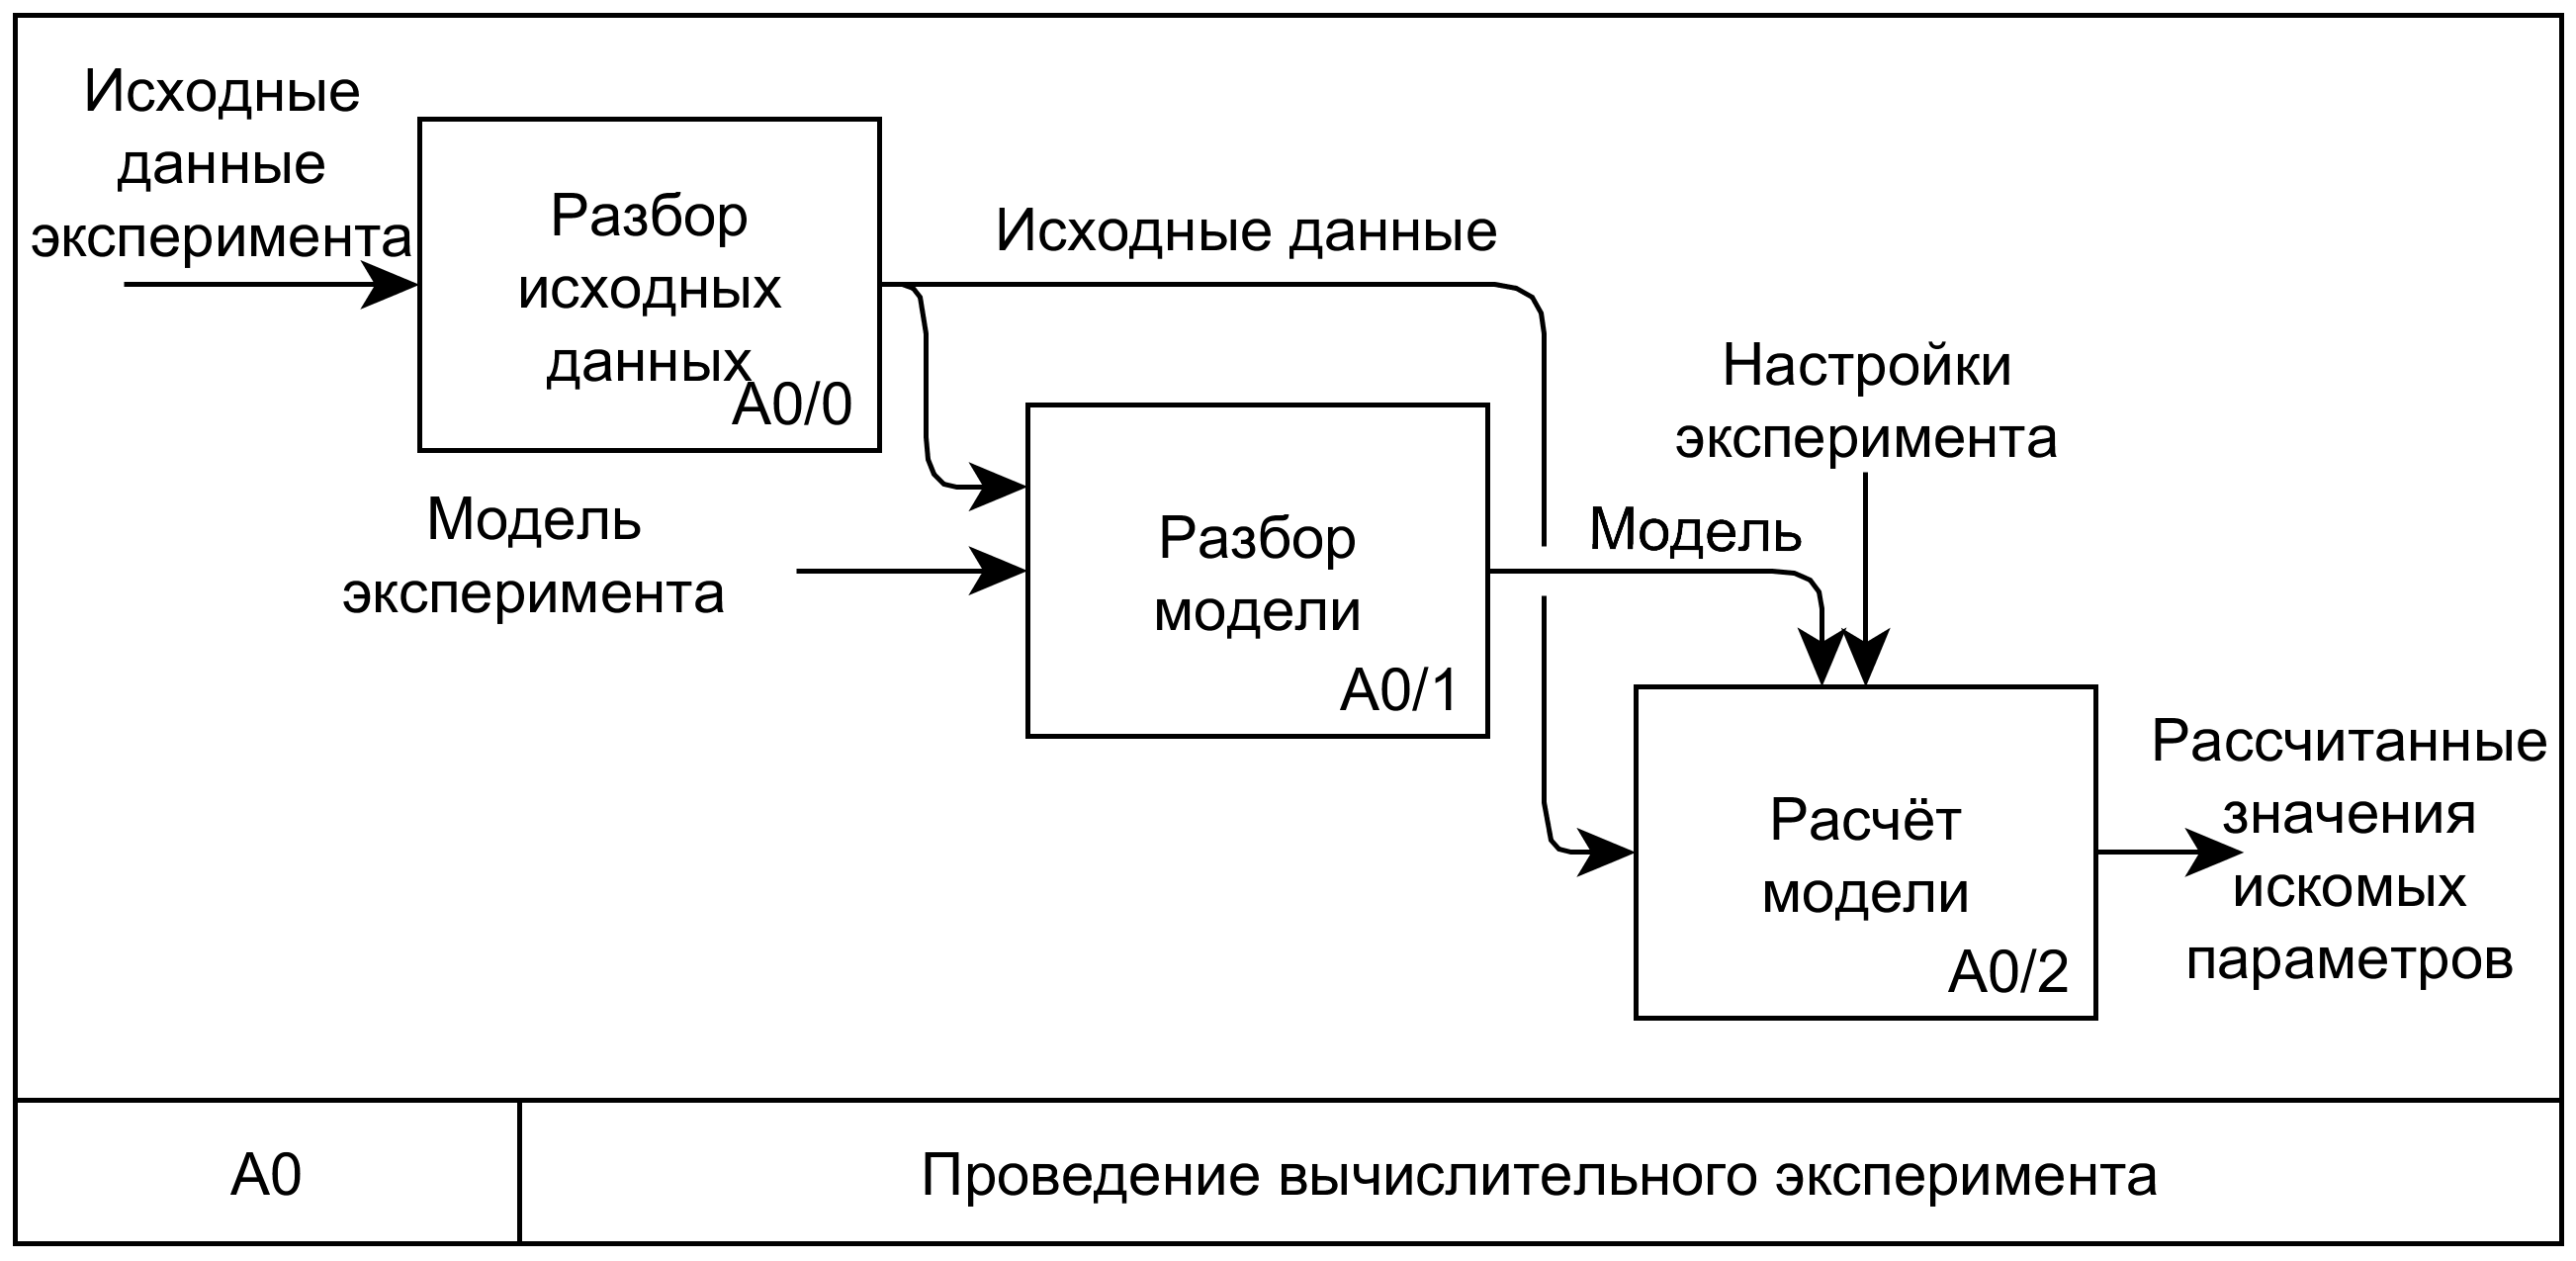
\includegraphics[width=.7\textwidth]{img/idef0/L1}
    \caption{Декомпозиция idef0-диаграммы верхнего уровня утилиты расчёта 
        модели}
    \label{fig:idef0-L1}
\end{figure}

\begin{figure}
    \centering
    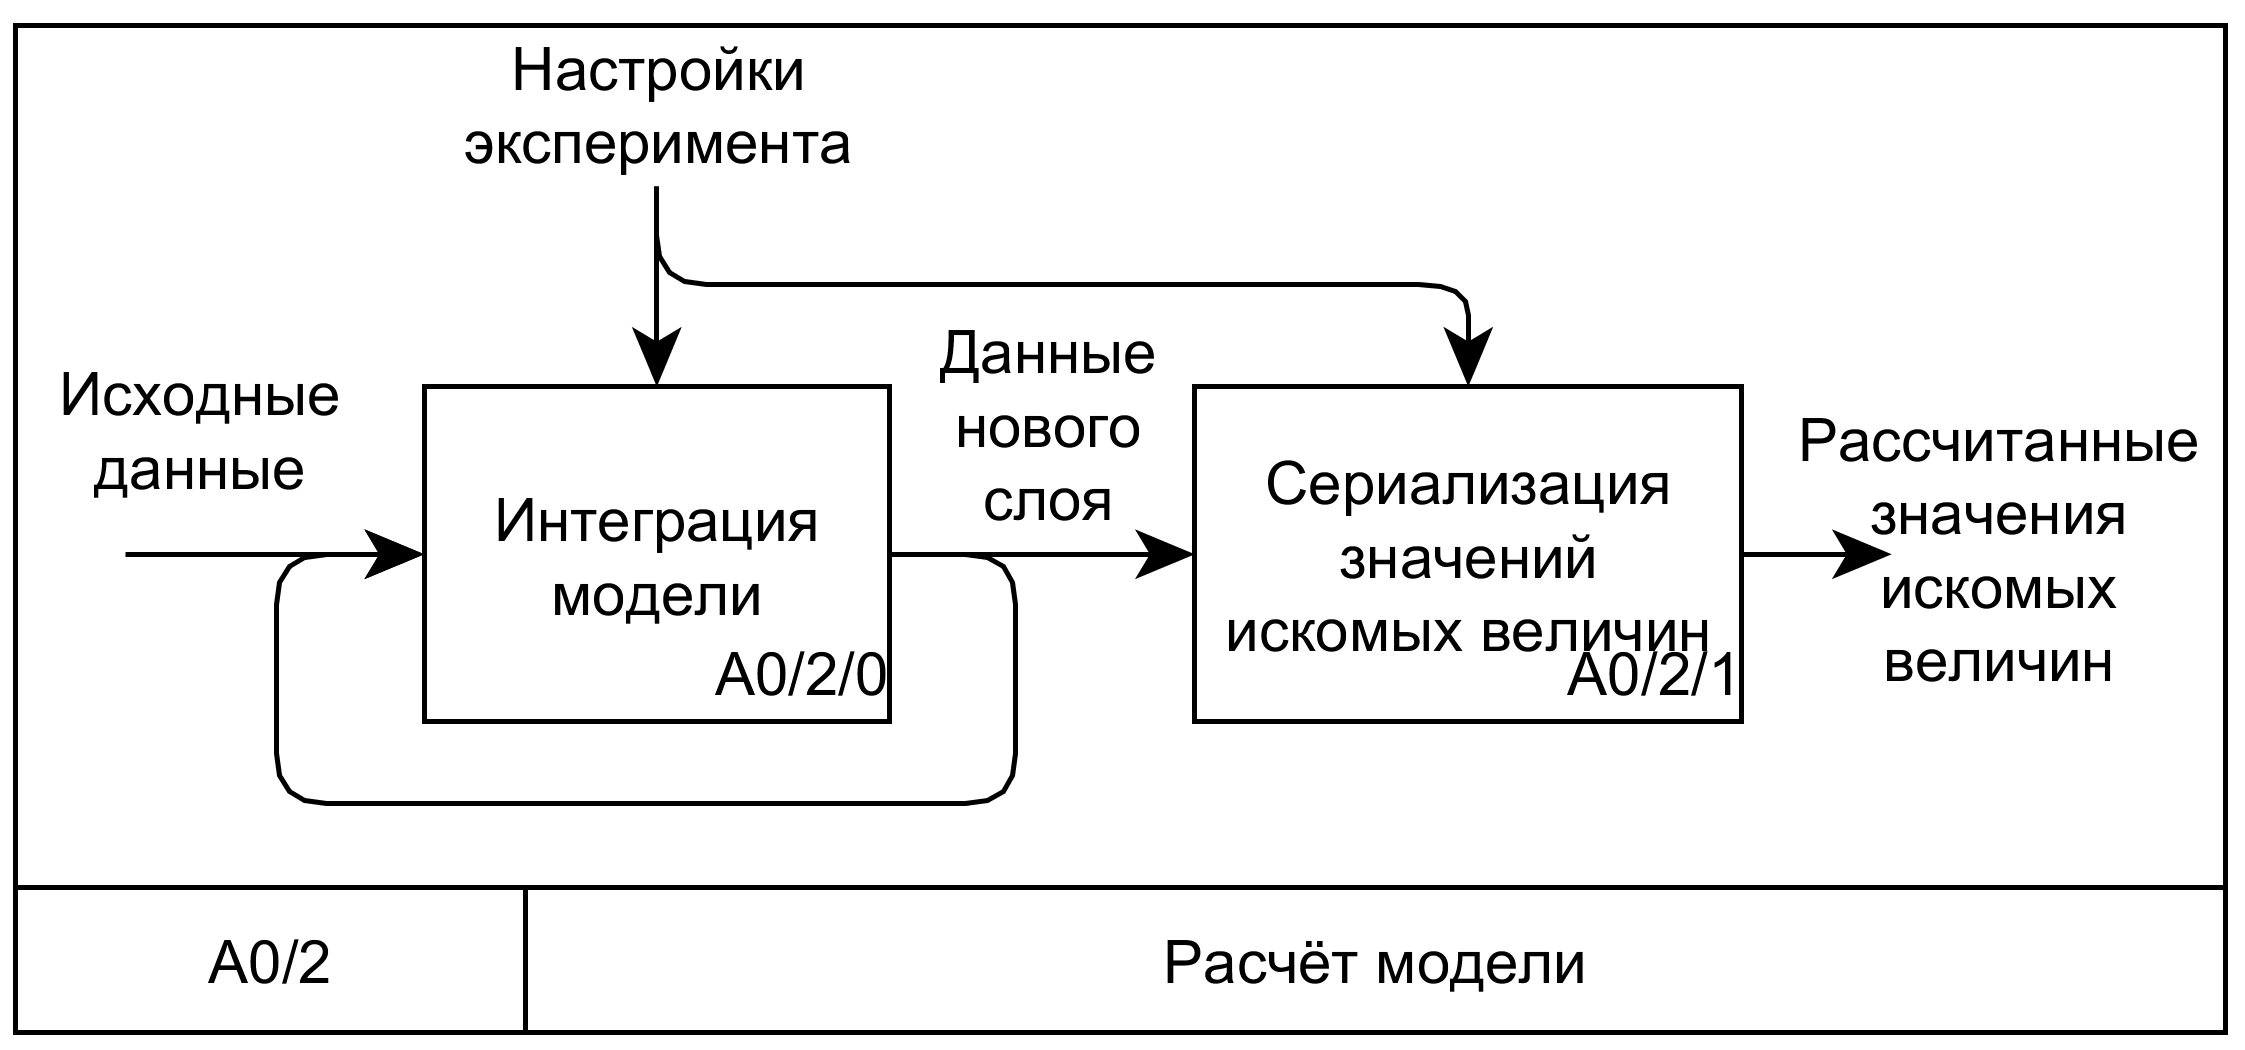
\includegraphics[width=.7\textwidth]{img/idef0/L2}
    \caption{Декомпозиция процесса расчёта модели}
    \label{fig:idef0-L2}
\end{figure}

\subsection{Библиотека математических подпрограмм}
Алгоритмы решения задач были вынесены в отдельную библиотеку PDELib. 
Разработанная библиотека предоставляет возможности:
\begin{itemize}
    \item Многомерной интерполяции с указанием типа интерполяции по каждой из 
    осей
    \item Переноса пространственных распределений скалярных величин в полярных 
    координатах между различными сетками
    \item Расчёта интегралов
    \begin{itemize}
        \item на равномерных сетках
        \item на неравномерных сетках
    \end{itemize}
    \item Решения обыкновенных уравнений
    \item Решения дифференциальных уравнений
    \begin{itemize}
        \item обыкновенных
        \item двумерных параболических в полярных координатах
        \item двумерных эллиптических в полярных координатах
    \end{itemize}
    \item Сериализации и десериализации представленных таблицами функций 
    нескольких переменных
    \item Визуализации трёхмерных данных в полярной системе координат в виде 
    теплокарт
\end{itemize}
Диаграмма классов библиотеки PDELib, за исключением изолированных классов, 
представлена на рисунке~\ref{fig:classDiagPdelib}.

\begin{sidewaysfigure}
    \centering
    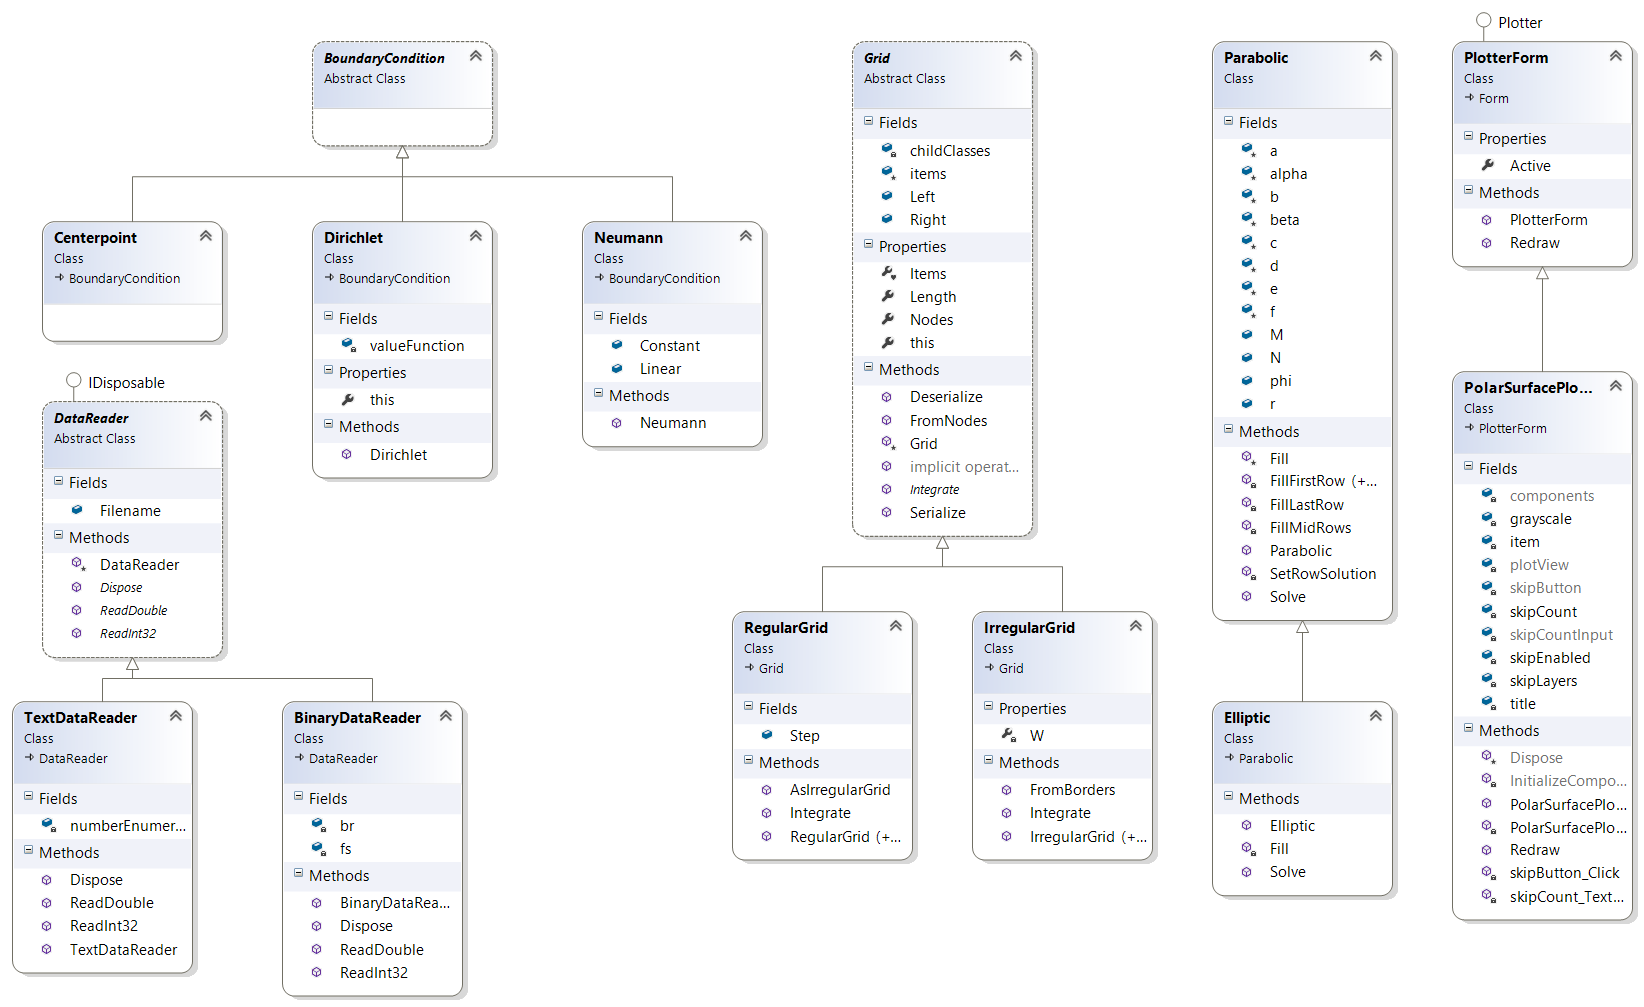
\includegraphics[width=\linewidth]{img/classDiag/pdelib}
    \caption{Диаграмма классов библиотеки PDELib}
    \label{fig:classDiagPdelib}
\end{sidewaysfigure}

\subsection{ПО для проведения численного эксперимента}
\subsubsection{Известные пользователю типы данных}
Для проведения вычислительного эксперимента пользователю необходимы такие типы 
данных, как скалярные величины, полярные распределения, функции для задания 
зависимостей между различными параметрами и сетки, определяющие расчётную 
область. Все эти типы данных вместе с примерами их использования приведены в 
таблице~\ref{tab:userData}.

\vspace{3cm}
\begin{table}[h]
    \caption{Известные пользователю типы данных}
    \centering
    \begin{tabu}{|L{2.5cm}|X[l]|L{5cm}|}
    	\hline
    	Тип данных & Описание & Пример значения \\ \hline
    	Scalar     & Числовое значение & Давление в области, напряжённость 
    	поля\\ \hline
    	Field      & Пространственное распределение числовых значений & 
    	Температура каждой точки области \\ \hline
    	Function   & Соотношение между параметрами & Заданная таблицей 
    	зависимость теплопроводности материала от его температуры \\\hline
        Grid & Сетка, задающая расчётные узлы на отрезке прямой & Разбиение 
        37мью узлами отрезка от $r=0$ до $r=3.5$ \\\hline
    \end{tabu}
    \label{tab:userData}
\end{table}

\clearpage

\subsubsection{Механизм расчёта модели}
В связи с отсутствием привязки метода счёта к конкретной вычислительной задаче, 
было необходимо разработать достаточно гибкий механизм счёта, позволяющий 
вычислять данные достаточно произвольной природы на основании конфигурируемых 
пользователем процессов. 

Спроектированный механизм выглядит следующим образом:
\begin{itemize}
    \item Модель состоит из данных и вычислительных блоков.
    \item Данные (сетки, поля, скалярные величины и именованные функции) 
    хранятся в глобальном хранилище, далее "контекст модели".
    \item Все данные могут быть вычислены с помощью "контекста исполнения".
    \item Контекст исполнения представляет собой хранилище для:
    \begin{itemize}
        \item локально переопределённых переменных;
        \item именованных индексов, соответствующих сетками в модели;
        \item параметры вызова именованной функции.
    \end{itemize}
    \item Вычислительные блоки модели определяют процесс расчёта
    \item Каждый вычислительный блок производит расчёт определённой неизвестной 
    величины. Тип рассчитываемого значения и дополнительная требуемая блоку 
    информация зависит от вида блока.
\end{itemize}

Каждый вычислительный блок реализует два метода: расчёта нового приближения 
неизвестного, и фиксации нового приближения. Такое разделение необходимо для 
возможности реализации расчётных блоков с состоянием (например, для реализации 
блока итерационного процесса).

\subsubsection{Вычисление выражений}
\paragraph{Контекст исполнения}
Для возможности одинаковым образом использовать в задающих модель выражениях 
констант и переменных разных типов (сетки, скалярные величины и поля скалярных 
величин) было введено понятие контекста исполнения. Контекст исполнения зависит 
от места, где встречается выражение. Контекст выполняет несколько важных 
функций.

Во-первых, если выражение используется в качестве инициализатора скалярного 
поля, либо является внутренним выражением спецфункции "integrate", либо 
определяет значение одного из параметров параболического или эллиптического 
выражения, то в контексте присутствуют именованные индексы, соответствующие 
сеткам $r$ и $\varphi$. В рамках такого контекста переменные, относящиеся к 
сеткам, будут соотвествовать хранимым по указанным индексам величинам. К 
примеру, символ переменной-сетки $r$ будет вычислится к радиусу каждой точки 
сетки, а символ переменной-поля $y$, вычислится к конкретному значению в каждой 
точке.

Во-вторых, наличие контекста позволяет реализовать локальное переопределение 
глобальных параметров. Это, в частности, важно для возможности реализации 
решения обыкновенных уравнений и для инициализации именованной функции 
выражением.

В-третьих, через контекст исполнения передаются аргументы вызова именованной 
функции. Примерами таких функций могут быть как предопределённые функции 
(арифметические операции, экспоненциирование и др), так и пользовательские 
(таблично заданная зависимость одного параметра от других).

\paragraph{Деревья выражений}
Для возможности вычисления заданных пользователем соотношений и выражений 
производится их разбор и преобразование в дерево выражений.

Дерево выражений состоит из узлов следующих видов:
\begin{itemize}
    \item Constant -- содержит некое числовое значение.
    \item Variable -- содержит имя переменной, по которому её можно найти в 
    контексте исполнения.
    \item FunctionCall -- содержит имя вызываемой функции и список выражений, 
    соответствующий её аргументам.
    \item IntegrationCall -- особый вид функции, соответствующий вычислению 
    интеграла. Введён из-за отличий в обработке контекста модели по сравнению с 
    FunctionCall (необходимо дополнение контекста вычисления 
    выражений-аргументов именованными индексами).
\end{itemize}

Все такие узлы могут быть вычислены при условии передачи в подпрограмму 
вычисления корректного контекста исполнения (для вычисления значения 
переменной-поля необходимо передать именованные индексы точки на этом поле, и 
т.д.). Диаграмма потоков данных при вычислении узла дерева выражений 
представлена на рисунке~\ref{fig:expressionDfd}.

\begin{figure}
    \centering
    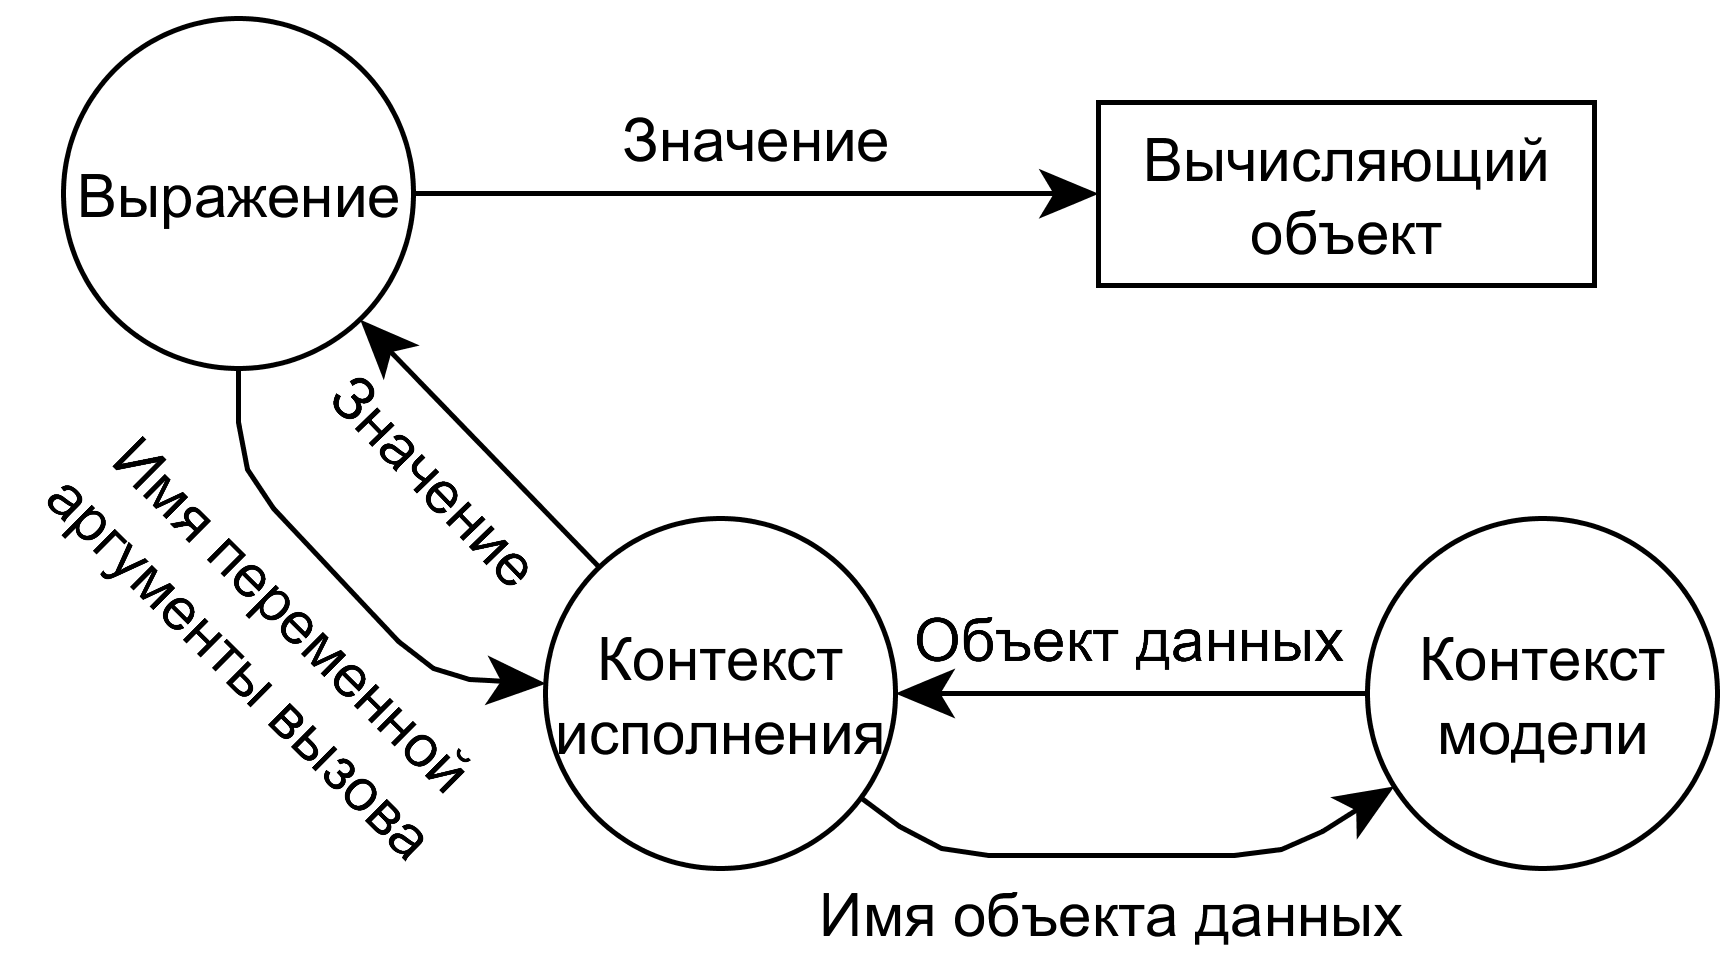
\includegraphics[width=.8\textwidth]{img/expression/dfd}
    \caption{Диаграмма потоков данных при вычислении узла дерева выражений}
    \label{fig:expressionDfd}
\end{figure}

\subsubsection{Вычислительные блоки модели}
Поведение модели определяеттся вычислительными блоками, из которых она состоит. 
Блоки реализуют различные механизмы расчёта какого-либо параметра - как решение 
дифференциальных уравнений, как решение обычных уравнений, как результат 
вычисления выражения и т.д.

На уровне всей модели расчёт происходит следующим образом: сначала все 
вычислительные блоки модели осуществляют шаг расчёта, после чего все блоки 
осуществляют шаг закрепления результата. Подобная двухшаговая структура расчёта 
позволяет включать в модель итерационные процессы.

Особенности реализации отдельных видов блоков описываются ниже.

\paragraph{Выражение}
Наиболее простой из вычислительных блоков. Осуществляет вычисление выражения и 
его запись в предоставленную переменную контекста модели. Если неизвестным 
является скалярное поле, то при вычислении в контексте исполнения также 
доступны скалярные поля и значения соответствующих узлов сеток.

\paragraph{Обыкновенное уравнение}
Блок, осуществляющий решение уравнения вида $f(x) = 0$. Указываются интервал 
поиска, требуемая точность решения и выражение $f(x)$ (на указанном интервале 
должно быть только одно решение). В контексте исполнения неизвестная переменная 
локально переопределена; корень уравнения записывается в контекст модели в 
качестве нового значения скалярной переменной.

\paragraph{Обыкновенное дифференциальное уравнение}
Блок, осуществляющий решение ДУ вида $\frac{\p y}{\p t} = k(t)y + c(t)$. 
Задаются функции $k(t)$ и $c(t)$, результат решения в очередной момент времени 
хранится в скалярной переменной, соответствующей неизвестному. В качестве 
метода решения используется метод Рунге-Кутта 4 порядка точности.

\paragraph{Параболическое дифференциальное уравнение}
Блок, осуществяющий решение параболического ДУ вида~(\ref{eq:parabolic}). 
Входными данными являются величины $A,B,C,D,U$; выходными - величина $\hat{U}$. 
Решение осуществляется построением полностью неявной разностной схемы на 
шаблоне типа "крест", описанной в разделе~\ref{sec:parabolic-scheme}, с 
последующим решением полученной схемы алгоритмом матричной прогонки.

\paragraph{Эллиптическое дифференциальное уравнение}
Блок, осуществяющий решение эллиптического ДУ вида~(\ref{eq:elliptic}). 
Входными данными являются величины $A,B,C,D$; выходными - величина $U$. 
Решение осуществляется аналогично решению параболического с описанными 
в~\ref{sec:parabolic-scheme} значениями специфичных для параболического 
уравнения полей.
 
\paragraph{Итерационный процесс}
Блок, позволяющий решать нелинейные версии различных уравнений. Входными 
данными такого блока являются максимальная относительная разница двух 
последовательных приближений, максимальное число итераций, имя неизвестной 
переменной и список дочерних ему вычислительных блоков, осуществляющих пересчёт 
данных. Опционально указывается коэффициент релаксации итерационного процесса и 
список связанных с неизвестной переменной величин. Такие опциональные величины 
также изменяются в ходе итерационного процесса; при их расчёте, как и при 
расчёте неизвестной переменной, учитывается коэффициент релаксации. Также 
указывается необходимость сброса нового приближения при начале итераций для 
расчёта данных на новом слое.

В дочерних блоках итерационного процесса для неизвестной переменной и каждой 
связанной переменной вводятся аналогичные им по типу переменные с именами, 
образованными добавлением к имени переменной постфикса "new" и хранящие текущее 
приближение значения соответствующей переменной на новом слое.

\paragraph{Определённый пользователем процесс}
Для реализации каких-либо специфических способов расчёта в ПО оставлена 
возможность использования определённых пользователем блоков. Хотя базовые блоки 
программы позволяют решать достаточно широкий спектр задач, необходимо заранее 
реализовать механизмы, позволяющие пользователю определить новый блок -- к 
примеру, реализующий особый алгоритм либо решающий узкоспециализированную 
задачу.

Определённый пользователем блок должен реализовывать методы:
\begin{itemize}
    \item Создания блока из записи с его настройками.
    \item Расчёта новых значений искомой величины.
    \item Фиксации новых значений искомой величины (требуется для блоков с 
    внутренним состоянием, таких как итеративные).
\end{itemize}

\subsubsection{Внутренние типы данных}
Таким образом, для реализации описанного выше механизма расчёта вводятся 
дополнительные типы:
\begin{itemize}
    \item ModelData -- базовый класс данных, составляющих состояние модели
    \begin{itemize}
        \item FunctionData -- хранит информацию о соотношениях (табличных и 
        заданных формулой)
        \item NumberData -- хранит информацию о скалярных величинах
        \item ArrayData -- хранит информацию о скалярных
        \item GridData -- хранит информацию о сетке
    \end{itemize}
    \item Expression -- базовый класс элемента деревьев выражений
    \begin{itemize}
        \item Constant -- узел дерева выражений, хранящий константу
        \item Variable -- узел дерева выражений, хранящий имя данных модели
        \item FunctionCall -- узел дерева выражений, соответветствующий 
        вычислению именованного соотношения
        \item IntegrationCall -- особый вид узла-вычислителя, соответствующий 
        расчёту пространственного интеграла в расчётной области
    \end{itemize}
    \item ModelContext -- содержит информацию о текущем состоянии модели
    \item ExecutionContext -- содержит информацию, необходимую для расчёта 
    вычисляемого выражения
    \item ModelBlock -- базовый класс вычислительных блоков модели, необходимых 
    для расчёта:
    \begin{itemize}
        \item Expression -- выражений
        \item DichotomyModelBlock -- обыкновенных уравнений
        \item OrdinaryModelBlock -- обыкновенных дифференциальных уравнений
        \item EllipticModelBlock -- двумерных эллиптических ДУ
        \item ParabolicModelBlock -- двумерных параболических ДУ
        \item IterativeModelBlock -- итерационных процессов
        \item CustomModelBlock -- определённых пользователем процессов
    \end{itemize}
\end{itemize}

Диаграмма классов, содержащая вышеприведённые типы и относящаяся к утилите 
PDESS, приведена на рисунке~\ref{fig:classDiagPdess}.

\begin{sidewaysfigure}
    \centering
    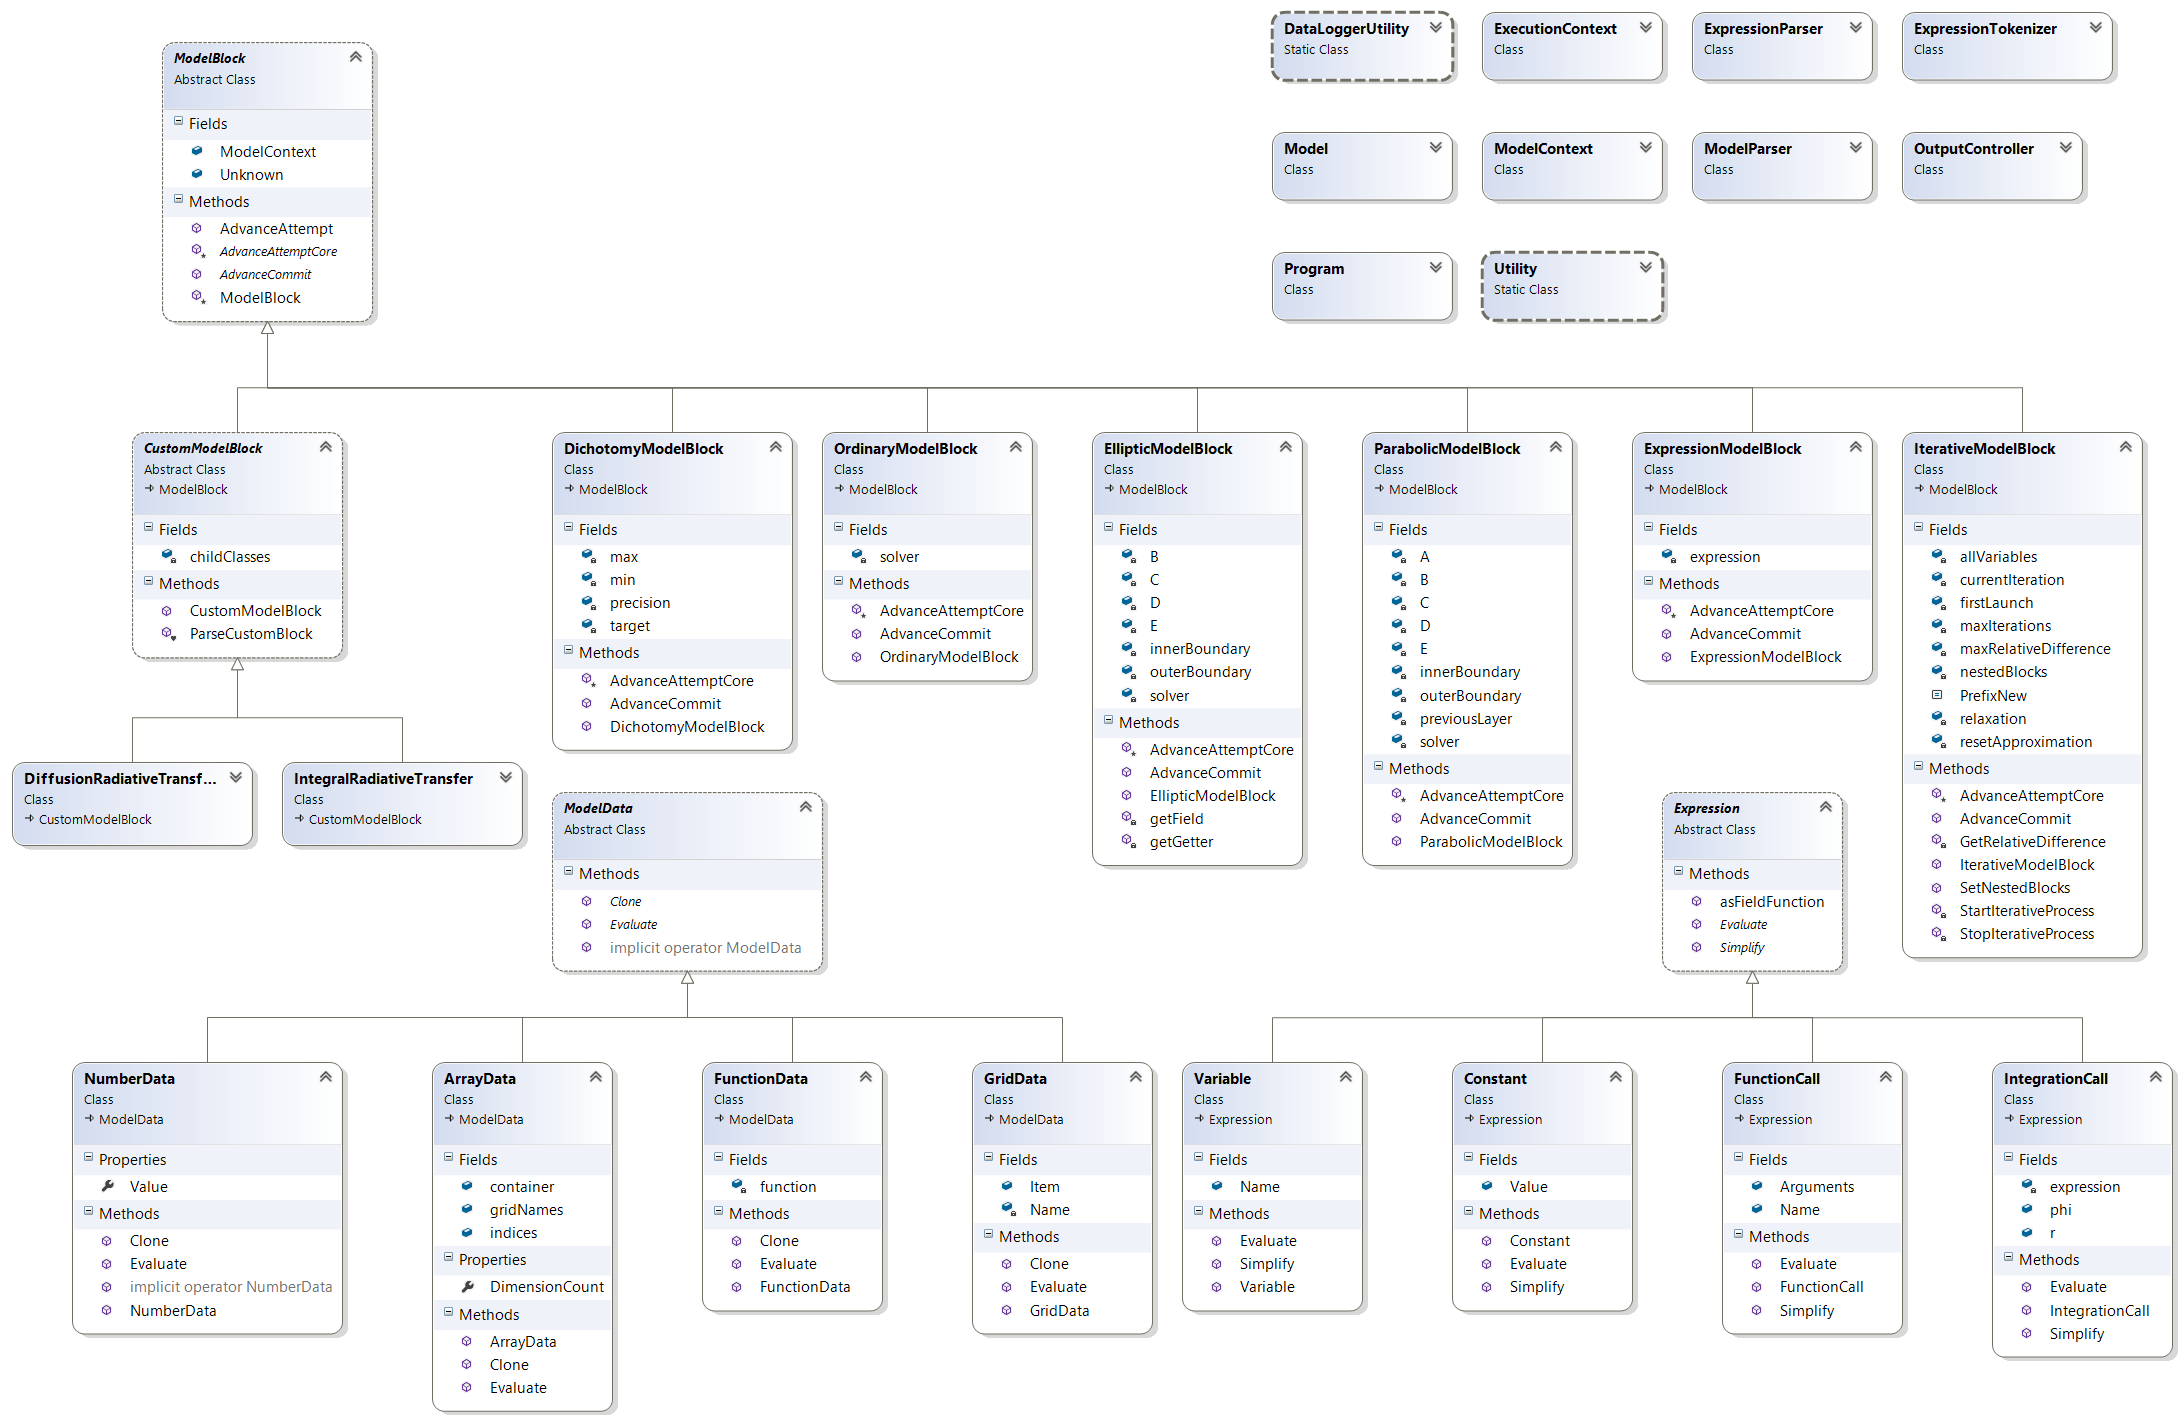
\includegraphics[width=\linewidth]{img/classDiag/pdess}
    \caption{Диаграмма классов утилиты PDESS}
    \label{fig:classDiagPdess}
\end{sidewaysfigure}

\subsubsection{Примеры реализации дополнительных видов блоков}
Для иллюстрации механизма использования определённых пользователем 
вычислительных блоков в качестве примера в рамках работы было реализовано два 
вида таких блоков -- блок расчёта переноса излучения в диффузионном приближении 
и в интегральной постановке.

Задача расчёта переноса излучения возникает при моделировании сильноизлучающих 
полупрозрачных сред, и может быть записана в форме~(\ref{eq:divFInt}). 
$U_\nu$ здесь рассчитывается из~(\ref{eq:luminInt}), где $U_\nu^{eq}, U_\nu$ -- 
равновесная и устанавливающаяся в среде спектральные объёмные плотности 
излучения, $k_\nu$ -- коэффициент оптического поглощения среды. Часто 
используется~\cite{gzl} диффузионное приближение~(\ref{eq:luminDiff}), вносящее 
погрешность порядка 15-35\%, но позволяющее свести задачу к решению набора 
эллиптических уравнений.

\begin{equation}
\begin{gathered}
    div F = \int_{0}^{\infty} div \vec{F_\nu} d\nu\\
    div \vec{F_\nu} = c k_\nu (T, p) (U_\nu^{eq}(T) - U_\nu)\\
    \label{eq:divFInt}
\end{gathered}
\end{equation}

\begin{equation}
    U_\nu = 
    \frac{1}{2\pi}
    \int_{0}^{2\pi}d\varphi
    \int_{0}^{\frac{\pi}{2}} sin(\theta)d\theta
    \int_{0}^{L'}k_\nu(l')U_\nu^{eq}(l')e^{-\int_{0}^{l'}k_\nu(l")dl"}dl'
    \label{eq:luminInt}
\end{equation}

\begin{equation}
    \vec{F_\nu} = - \frac{c}{3 k_\nu(T, p)} \nabla U_\nu
    \label{eq:luminDiff}
\end{equation}

\paragraph{Перенос излучения в диффузионном приближении}
Объединение уравнений~(\ref{eq:divFInt}) и~(\ref{eq:luminDiff}) даёт 
уравнение~(\ref{eq:luminDiffElliptic}), эквивалентное~(\ref{eq:elliptic}) при 
условии $B = \frac{1}{3 k_\nu}, C = 0, D = k_\nu, E = k_\nu U_\nu^{eq}$.

\begin{equation}
    - div(\frac{1}{3k_\nu} \nabla U_\nu) + k_\nu U_\nu = k_\nu U_\nu^{eq}
    \label{eq:luminDiffElliptic}
\end{equation}

Поскольку для расчёта интеграла~(\ref{eq:divFInt}) необходимо решать целый 
пакет подобных задач, критически важно получить любое возможное ускорение 
счёта. Один из способов ускорения - разбить такой пакет задач на несколько 
пакетов поменьше, и решать набор таких пакетов параллельно. Такой подход 
привлекателен ещё и потому, что он ограничивает число одновременно решаемых 
задач реальной возможной степенью распараллеливания счёта -- это важно, так как 
алгоритм матричной прогонки, применяющийся для решения эллиптических уравнений, 
требует достаточно большого количества памяти ($O(n^{1.5})$, где $n$ - 
количество узлов сетки).

Блок-схема алгоритма решения задачи переноса излучения представлена на 
рисунке~\ref{fig:flowchartLuminDiff}.

\begin{figure}
    \centering
    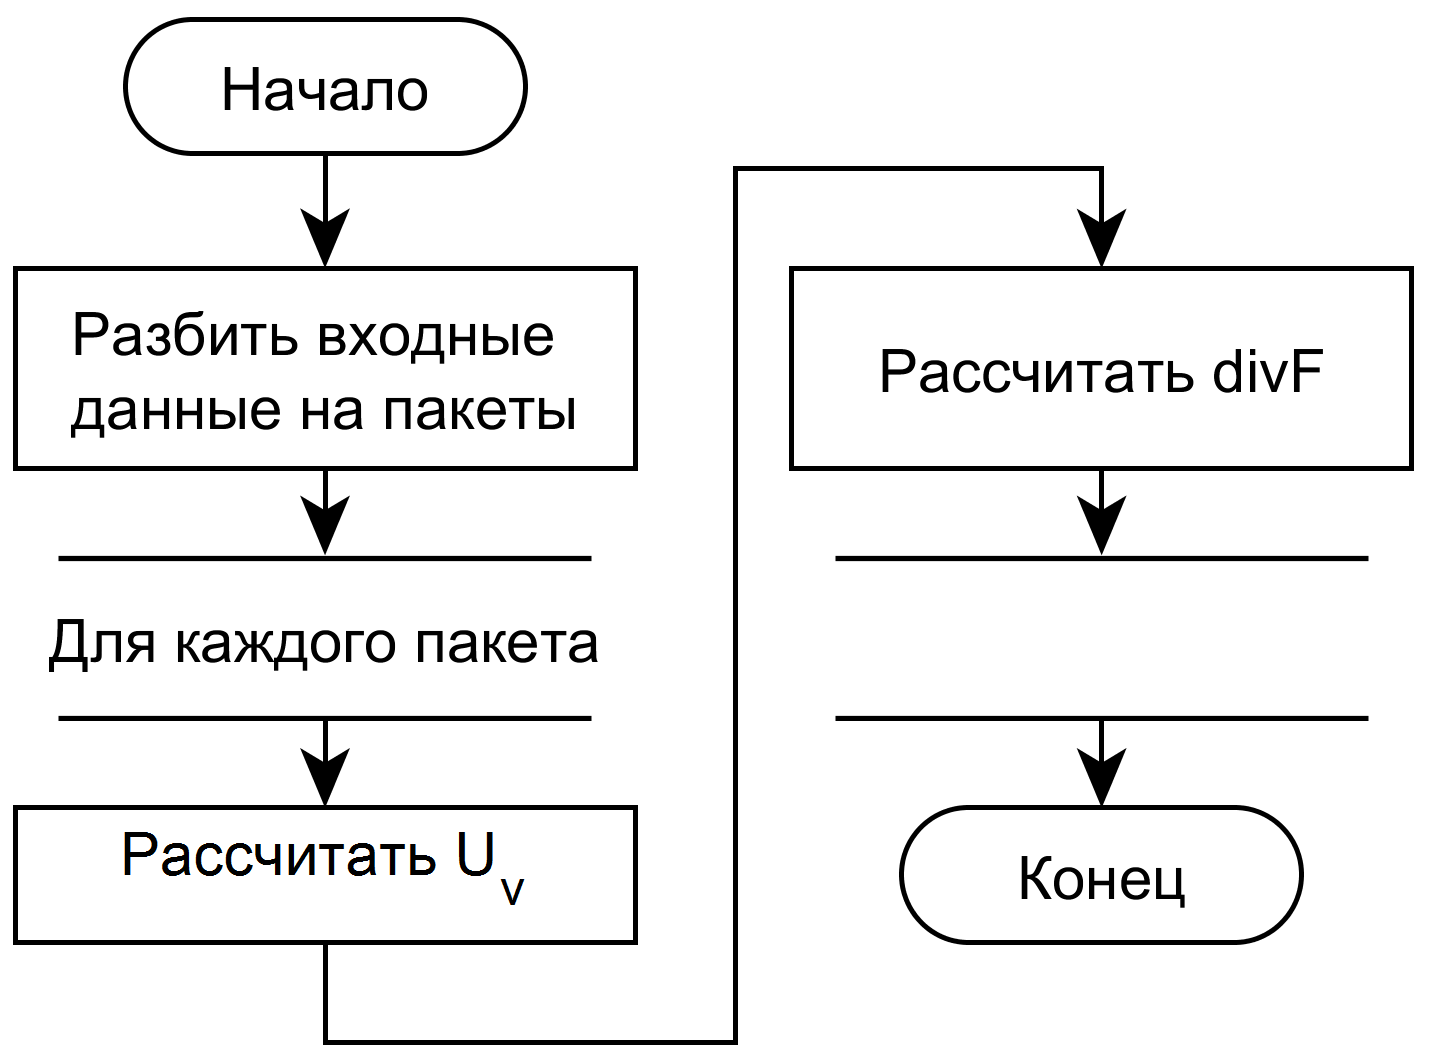
\includegraphics[width=.5\linewidth]{img/flowchart/luminDiff}
    \caption{Блок-схема алгоритма решения задачи переноса излучения}
    \label{fig:flowchartLuminDiff}
\end{figure}

\paragraph{Перенос излучения в интегральной постановке}\label{sec:intSolver}
Для решения задач, чувствительных к погрешностям диффузионного приближения, 
возможен расчёт переноса излучения в её исходной 
постановке~(\ref{eq:luminInt}), обозначения проиллюстрированы на 
рисунке~\ref{fig:ray3d}.

Несмотря на то, что прямой расчёт интеграла вычислительно более сложен, чем 
расчёт диффузионного приближения, при расчёте двумерной задачи он обладает 
некоторыми особенностями, позволяющими воспользоваться средствами 
видеоускорителей для своего эффективного счёта.

Во-первых, процесс расчёта интеграла является алгоритмически значительно более 
простой задачей, нежели расчёт СЛАУ, что позволяет уложиться в малое число 
регистров, доступных процедуре при выполнении на графическом ускорителе. 
Во-вторых, при расчёте интеграла дополнительной памяти требуется значительно 
меньше, и она преимущественно лишь читается, в отличии от алгоритма решения 
СЛАУ, что позволяет сократить использование общей, медленной память 
видеоускорителя. В-третьих, расчёт интеграла можно производить отдельно для 
разных точек сетки, тем самым на порядки повышая число независимых параллельно 
выполняющихся потоков. В-четвёртых, общие для различных точек данные, 
необходимые для расчёта -- такие, как $U_\nu^{eq}, k_\nu$ и шаблоны 
интегрирования -- могут храниться в кеше константной памяти, тем самым сокращая 
количество обращений к медленной общей памяти графического процессора. Все эти 
черты делают интегральную постановку задачи расчёта переноса излучения 
привлекательной с точки зрения производительности по сравнению с диффузионным 
приближением.

Для значительного сокращения вычислений необходимо выполнить некоторые 
преобразования интеграла~\eqref{eq:luminInt}. Для фиксированных $\varphi$, 
$\theta$ и расчётной точки, подынтегральное выражение соответствует 
распространению излучения вдоль луча $\vec{L'}$, где координата $0$ 
соответствует расчётной точке, а $L'$ - точке пересечения луча с границей 
расчётной области (рисунок~\ref{fig:ray3d}). Для взятия интеграла из каждой 
точки испускается $Q$ таких лучей, с интервалами $\Phi = \frac{PI}{Q}$ между 
ними. Пример шаблона интегрирования для конкретной точки приведён на 
рисунке~\ref{fig:intpattern}.

\begin{figure}
    \centering
    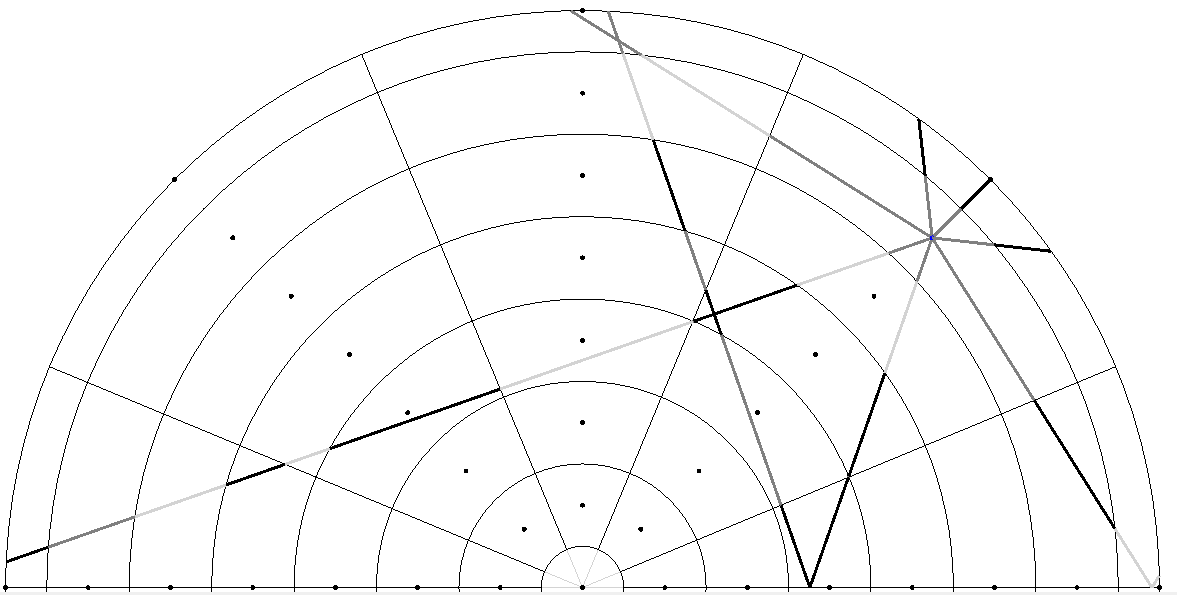
\includegraphics[width=.5\linewidth]{img/luminInt/intpattern}
    \caption{Шаблон интегрирования точки (2, 7) на сетке размером $8 \times 5$. 
    Используется 7 лучей на точку}
    \label{fig:intpattern}
\end{figure}

В проекции луча на расчётную плоскость, с учётом симметрии разряда относительно 
оси "центр разряда -- центр области", луч разбивается ячейками на сегменты, 
соответствующие ячейкам сетки, через которые проходит луч. Далее считается, что 
луч состоит из $N$ сегментов, каждому из которых соответствует ширина сегмента 
$w_i$, координата начала сегмента на луче $r_i$, спектральная объёмная 
плотность излучения $U_i$ и коэффициент оптического поглощения $k_i$, значения 
которых соответствуют значениям в точке, образующей ячейку сетки, пересекаемую 
данным сегментом луча. 
Пример разбиения для одного луча показан на рисунке~\ref{fig:ray2d}. Подобные 
разбиения строятся для каждого луча интегрирования, для каждой точки сетки 
однажды до начала вычислений, и нуждаются в перестройке только при изменении 
геометрии сетки. 

\begin{figure}
    \centering
    \begin{minipage}{.48\linewidth}
        \centering
        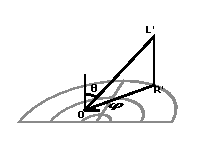
\includegraphics[width=\linewidth]{img/luminInt/ray}    
        \caption{Луч интегрирования для трёхмерной задачи}
        \label{fig:ray3d}
    \end{minipage}
    \hfil
    \begin{minipage}{.48\linewidth}
        \centering
        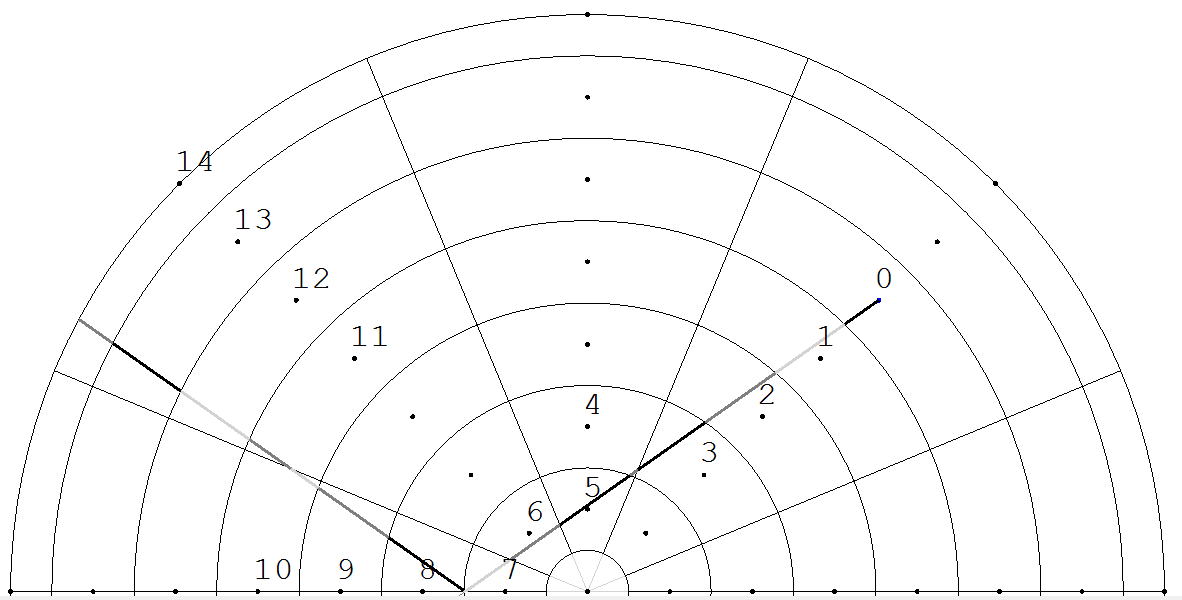
\includegraphics[width=\linewidth]{img/luminInt/intsingle}    
        \caption{Разбитый сеткой на сегменты луч интегрирования для двумерной 
        задачи. Пронумерованы образующие пересекаемые лучом ячейки точки}
        \label{fig:ray2d}
    \end{minipage}
\end{figure}

Поскольку задача является двумерной, необходимо избавиться от интеграла по 
$\theta$. 
Для этого интеграл~\eqref{eq:luminInt} проецируется на расчётную плоскость 
задачи, с учётом замены $l sin(\theta) = r$, где $l$ -- координата на луче 
интегрирования, а $r$ -- координата на проекции этого луча на расчётную 
плоскость задачи. Здесь и далее расчёты ведутся для одного луча, 
соответствующего фиксированному значению $\varphi$ в ходе вычисления 
интеграла~\eqref{eq:luminInt}.

\begin{gather*}
\int_{0}^{\frac{\pi}{2}} sin(\theta)d\theta
\int_{0}^{L}k(l')U(l')e^{-\int_{0}^{l'}k(l")dl" }dl'  = \\
=\int_{0}^{\frac{\pi}{2}} d\theta
\int_{0}^{R}k(r')U(r')e^{-\int_{0}^{r'}k(r")dr" csc(\theta)}dr' =\\ 
=\int_{0}^{\frac{\pi}{2}} d\theta
\sum_{i=0}^{N-1} U_i k_i 
\int_{0}^{w_i} 
e^{-\sum_{j=0}^{i-1}k_j w_j csc(\theta)} e^{-k_i r' csc(\theta)}dr' =
\end{gather*}

Замена: $e^{-\sum_{j=1}^{i-1}k_j w_j} = c_i$

\begin{gather*}
=\int_{0}^{\frac{\pi}{2}} d\theta
\sum_{i=0}^{N-1} U_i k_i \int_{0}^{w_i} 
c_i^{csc(\theta)} e^{-k_i r' csc(\theta)}dr'  =\\  
=\int_{0}^{\frac{\pi}{2}} d\theta
\sum_{i=0}^{N-1} U_i k_i \frac{1}{k_i csc(\theta)}\int_{0}^{k_i w_i csc(theta)} 
c_i^{csc(\theta)} e^{-z}dz  =\\                  
=\sum_{i=0}^{N-1} U_i 
\int_{0}^{\frac{\pi}{2}} sin(\theta)d\theta
\int_{0}^{k_i w_i csc(theta)} 
c_i^{csc(\theta)} e^{-z}dz  =
\end{gather*}

Замена: $k_i w_i = a_i$

\begin{gather*}
=\sum_{i=0}^{N-1} U_i 
\int_{0}^{\frac{\pi}{2}} c_i^{csc(\theta)} sin(\theta)d\theta
\int_{0}^{a_i\ csc(\theta)} e^{-z}dz  =\\             
=\sum_{i=0}^{N-1} U_i 
\int_{0}^{\frac{\pi}{2}} c_i^{csc(\theta)} sin(\theta)d\theta
(1 - e^{-a_i\ csc(\theta)}) =\\    
=\sum_{i=0}^{N-1} U_i 
(
\int_{0}^{\frac{\pi}{2}} c_i^{csc(\theta)} sin(\theta)d\theta
-\int_{0}^{\frac{\pi}{2}} (c_ie^{-a_i})^{csc(\theta)} sin(\theta)d\theta
)
\end{gather*}

Таким образом получаем, что интеграл~\eqref{eq:luminInt}, с учётом взятия 
интеграла по $\varphi$ численно $Q$ лучами, испускаемыми из расчётной точки 
через каждые $\frac{2\pi}{Q}$ рад., с учётом разбиения каждого луча на $N(q)$ 
сегментов с шириной, спектральным потоком и оптической плотностью $w_i$, $U_i$ 
и $k_i$ соответственно, и с учётом замены  $f(x) = \int_{0}^{\frac{\pi}{2}} 
x^{csc(\theta)} sin(\theta)d\theta$, принимает вид
\begin{equation}
\frac{1}{Q}
\sum_{q=0}^{Q-1}
\sum_{i=0}^{N-1} U_i 
(f(c_i)-f(c_i e^{-a_i}))
\end{equation}
где $a_i = k_i w_i$ и $c_i = e^{-\sum_{j=1}^{i-1}a_j}$.
Поскольку ввиду $0<c_i\le1$ и $a_j\ge0$ выражение $c_i e^{-a_j}$ может 
принимать только значения из интервала $(0, 1]$, достаточно рассчитать функцию 
$f$ именно на этом интервале. График функции $f$ представлен на 
рисунке~\ref{fig:fplot}. В ходе вычислений функция $f$ была приближена 
полиномом 9 степени с центром разложения в $0.5$. Степень полинома выбиралась 
как наибольшая поместившаяся в оставшиеся после реализации алгоритма регистры 
вычислительного блока.

\begin{figure}
    \centering
    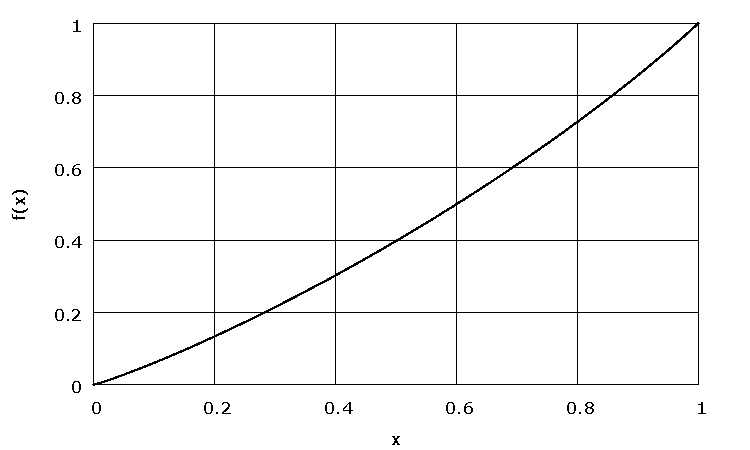
\includegraphics[width=.5\linewidth]{img/luminInt/fdata}
    \caption{График функции $f(x) = \int_{0}^{\frac{\pi}{2}} x^{csc(\theta)} 
    sin(\theta)d\theta$ на интервале $[0, 1]$}
    \label{fig:fplot}
\end{figure}

Собственно алгоритм интегрирования состоит из нескольких этапов. На первом, 
подготовительном этапе, выполняющемся однажды до начала вычислений, 
осуществляется построение разбиения лучей интегрирования на сегменты. Структуры 
данных формируются следующим образом: для сетки размера $N \times M$, с 
использованием $Q$ лучей, строится таблица дескрипторов лучей размера $N\times 
M \times Q$, содержащая в каждой строке число сегментов в данном луче, и номер 
первого сегмента в таблице сегментов. Каждый элемент таблицы сегментов содержит 
информацию о ширине сегмента и указатель на элемент массивов, содержащих данные 
о спектральной плотности излучения и оптической плотности ксенона в ячейке, 
соответствующей данному сегменту.
Схема адресации представлена на рисунке~\ref{fig:address}. 

\begin{figure}
    \centering
    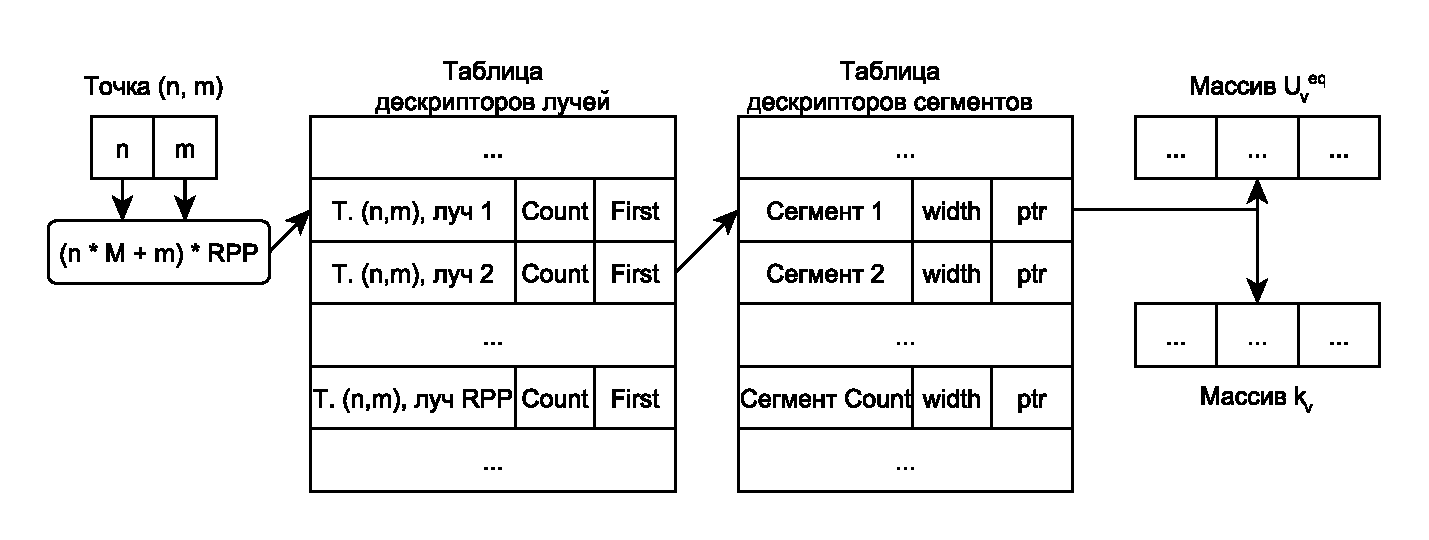
\includegraphics[width=\linewidth]{img/luminInt/address}
    \caption{Схема адресации таблиц дескрипторов лучей и их сегментов. RPP - 
    число лучей в шаблоне интегрирования каждой точки}
    \label{fig:address}
\end{figure}

Типы выбирались следующим образом: физические величины $k_\nu, U_\nu^{eq}, 
U_\nu$ имеют тип \lstinline[language=c]|float|, из-за того, что устройства 
вычислений с плавающей запятой двойной точности являются внешними устройствами 
для использованного видеоускорителя (NVIDIA GeForce GTX 770), и их 
использование снижает производительность на порядок и больше. Число сегментов 
на луч в дескрипторе луча имеет тип \lstinline[language=c]|short|, такой же тип 
имеет и указатель дескриптора сегмента на ячейку в массивах $k_\nu, 
U_\nu^{eq}$. Указатель на дескриптор первого сегмента в дескрипторе луча имеет 
тип \lstinline[language=c]|int|. Таким образом, для хранения информации о 
задаче необходимо $3 \times M \times N \times \sizeof(float) = 12MN$ байт для 
хранения профилей оптической плотности, исходящей из точки спектральной 
объёмной плотности излучения и вычисляемой падающей; плюс дополнительно 
$(\sizeof(short)+\sizeof(int))\times M \times N \times Q = 6MNQ$ байт для 
хранения таблицы дескрипторов лучей, плюс зависящее от конфигурации сетки 
количество памяти для хранения таблицы дескрипторов сегментов. Эксперименты 
показали значительное потребление памяти на хранение этой таблицы. Возможна 
модификация алгоритма, оперирующая максимальным количеством сегментов на луч и 
загрубляющая лучи с избыточным числом сегментов, что позволит свести 
потребление памяти на хранение лучей до $O(M\times N \times R_{PP} \times 
SPR_{max})$, где $R_{PP}$ -- число лучей в шаблоне интегрирования каждой точки, 
а $SPR_{max}$ -- максимальное число сегментов в луче.

На втором этапе алгоритма выполняются непосредственно вычисления. Входной пакет 
данных разбивается на блоки задач по $B$ потоков (соответствующих отдельным 
точкам) в каждом (по умолчанию $B=256$), и эти блоки задач отправляются на 
выполнение на мультипроцессоры графического ускорителя. Блок-схема алгоритма 
вычисления профиля $U_\nu$ интегральным методом приведена на 
рисунке~\ref{fig:flowchart}.

\begin{figure}
    \centering
    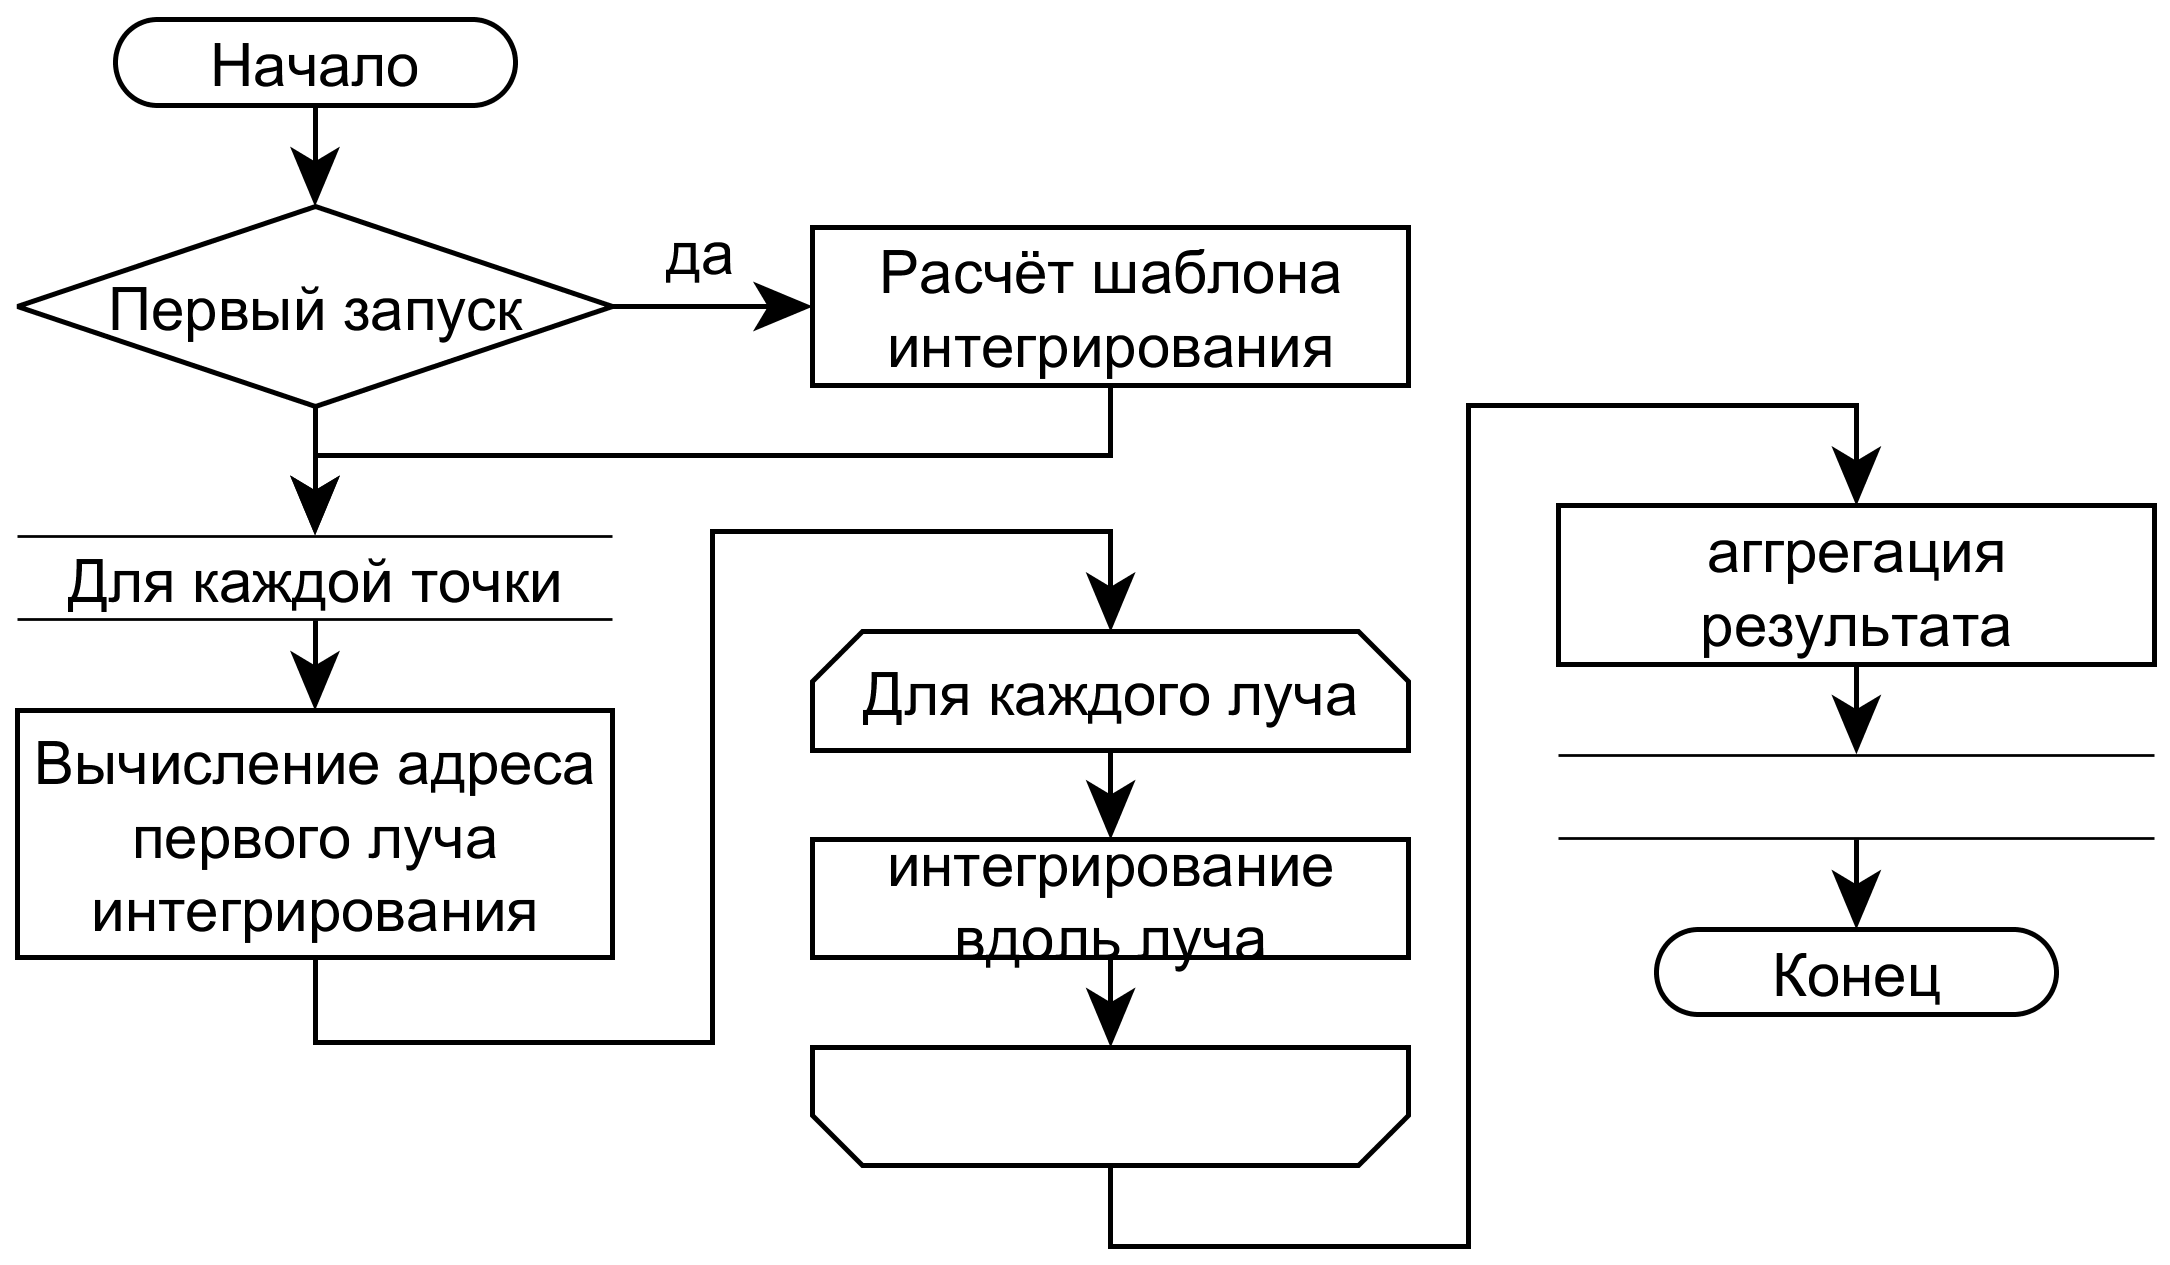
\includegraphics[width=.9\linewidth]{img/luminInt/flowchartint}
    \caption{Блок-схема алгоритма вычисления профиля $U_\nu$ методом 
    интегрирования}
    \label{fig:flowchart}
\end{figure}

При реализации алгоритма учитывались некоторые особенности архитектуры CUDA 
Kepler. Во-первых, указатели на профили $k_\nu, U_\nu^{eq}$ и на таблицы 
дескрипторов лучей и сегментов лучей передавались в вычислительную функцию с 
модификаторами \lstinline[language=c]|const __restrict__|, что позволяет 
использовать read-only кэш для двух-трёхкратного ускорения доступа к 
памяти\cite{cudaptr}.
Во-вторых, учтывался тот факт, что с ограничением в $65536$ регистров на 
потоковый мультипроцессор, для работы максимального ($2048$) количества потоков 
на мультипроцессоре необходимо, чтобы каждый поток использовал максимум $32$ 
регистра.
Тестирование алгоритма описано в~\cite{integral}.

\subsection{Вывод}
Обосновано разбиение проектируемого ПО на набор утилит. В текстовом виде и при 
помощи диаграмм idef0, dfd, блок-схем и диаграмм классов описан функционал 
отдельных частей разрабатываемых программ. Описаны реализованные расчётные 
блоки и механизмы их функционирования. В качестве примера определённого 
пользователем вычислительного блока приведены блоки и реализуемые ими алгоритмы 
расчёта задачи переноса излучения в диффузионном приближении силами ЦП и в 
интегральной постановке с применением технологии CUDA.

\section{Технологический раздел}
\subsection{Введение}
В данном разделе производится выбор языка программирования и сопутствующих 
программных средств. Описываются основные моменты программной реализации, 
методика тестирования и интерфейс ПО.

\subsection{Выбор языка программирования}
В качестве языка программирования был выбран язык C\#. Согласно экспериментам 
\cite{csharp_speed_comparison}, C\# обеспечивает такую же скорость исполнения 
кода, как и C, в тестах на скорость работы циклов и на скорость вычисления 
математических операций. Работа с массивами и матрицами в языке C\# медленнее, 
чем в языке C, в 4.5 раза, но данное отставание можно сократить до 1.7 раз при 
использовании unsafe-конструкций языка C\#. В обмен на потерю скорости, C\# 
предлагает значительно более удобные средства отладки, нежели языки C / C++, а 
также, обладая сборщиком мусора, практически исключает утечки памяти. Также 
платформа .NET обладает богатыми средствами создания легковесных потоков 
вычисления операций (к примеру, Parallel.For\cite{csharp_msdn_parallel}), что 
на многопроцессорных либо многоядерных системах даёт значительный прирост 
производительности. Также следует отметить, что в случае необходимости 
дальнейшего увеличения скорости исполнения кода, С-подобный синтаксис языка C\# 
и средства межъязыкового взаимодействия платформы .NET оставляют возможность 
относительно легко вынести все математические подпрограммы в библиотеки на 
языке C с минимальными изменениями. Данный подход хорошо 
проработан\cite{csharp_interop_A, csharp_interop_B} и потому выбор языка C\# 
является оправданным, так как позволяет ускорить разработку ПО без 
значительного ограничения производительности.

\subsection{Выбор программных средств}
В связи с выбором языка программирования и ограничением на платформу разработки 
как Windows 8, были выбраны программные средства, используемые при подготовке 
работы. Полный список средств, их версий и назначений предоставлен в 
таблице~\ref{tab:software}.

\begin{table}[h]
    \caption{Использованные при разработке программные средства}
    \centering
    \begin{tabu}{|>{\centering}p{3.5cm}|>{\centering}p{2.3cm}|X[c]|}
    	\hline
    	Название                         & Версия           & 
    	Назначение                                                \\ \hline
    	MS Visual Studio 2015 Enterprise & 14.0.25123.00 U2 & Среда разработки 
    	ПО                                       \\ \hline
    	TortoiseHG                       & 2.10             & Контроль версий 
    	(в сочетании с ресурсом bitbucket.org)    \\ \hline
    	TexStudio                        & 2.11.0           & Подготовка 
    	документации)                                  \\ \hline
    	yED                              & 3.14.1           & Создание 
    	схем                                             \\ \hline
    	TikzEdt                          & 0.2.3.0          & Создание 
    	иллюстраций                                      \\ \hline
    	gnuplot                          & 4.6 p4           & Визуализация 
    	результатов экспериментов                    \\ \hline
    	Notepad++                        & 6.5.1            & Текстовый 
    	редактор \\ \hline
    \end{tabu}
    \label{tab:software}
\end{table}

\subsection{Входные данные}
\subsubsection{Конфигурационный файл эксперимента}
Эксперимент описывается конфигурационным файлом, представляющим собой текстовый 
файл с json-объектом внутри. 

Все пути в конфигурационном файле записываются относительно его расположения.

Объект верхнего уровня имеет следующую структуру:

\begin{itemize}
    \item \textbf{settings} -- поле, хранящее json-объект, содержащий общие 
    настройки модели
    \item \textbf{variables} -- поле, хранящее json-объект с полями, 
    соответствующими переменным эксперимента
    \item \textbf{blocks} -- поле, хранящее json-массив, содержащий описание 
    вычислительных блоков эксперимента
    \item \textbf{output} -- поле, хранящее json-массив, содержащий имена 
    выходных переменных эксперимента
\end{itemize}

\paragraph{Настройки модели.} Секция \textbf{settings} содержит общие настройки 
модели. Синтаксис секции имеет следующую структуру:
\begin{itemize}
    \item \textbf{r-max} -- внешний радиус области моделирования
    \item \textbf{r-steps} -- количество шагов радиальной сетки
    \item \textbf{phi-steps} -- количество шагов тангенциальной сетки
    \item \textbf{time-step} -- шаг моделирования по времени
    \item \textbf{time-max} -- время, до которого производится моделирование    
\end{itemize}

\paragraph{Переменные эксперимента.} Секция \textbf{variables} описывает 
переменные, используемые в эксперименте. Запись, соответствующая определённой 
переменной, выглядит как поле json-объекта с именем, равным имени переменной, и 
значением, являющимся json-объектом с описанием значения переменной. Пример 
описания переменной, соответствующей именованной функции, приведён в листинге 
на рисунке~\ref{fig:lstVariable}.

\begin{figure}
    \centering
    \begin{lstlisting}[language=java,frame=single,numbers=left,breaklines=true]
"knu_p_t_nu":
{
    "type":"function",
    "initializer":"file",
    "filename":"data/knu_p_t_nu.txt",
    "interpolators":["exponential","exponential","linear"]
},
    \end{lstlisting}
    \caption{Описание переменной, соответствующей именованной скалярной функции 
    трёх аргументов}
    \label{fig:lstVariable}
\end{figure}

Описательные json-объекты, прежде всего, включают в себя дискриминатор типа 
\textbf{type}. 
Остальные поля в зависимости от типа имеют следующий синтаксис:
\begin{itemize}
    \item \textbf{scalar} -- скалярная величина
    \begin{itemize}
        \item \textbf{expression} -- содержит выражение, инициализирующее 
        переменную
    \end{itemize}
    \item \textbf{field} -- двумерное скалярное поле, определённое на области 
    решения задачи.
    \begin{itemize}
        \item \textbf{initializer} -- дескриптор инициализатора. Допустимые 
        значения - \textbf{expression}, \textbf{file}
        \item \textbf{expression} -- выражение, использующееся в 
        инициализаторе. При расчёте в контексте исполнения доступны индексы 
        скалярных полей и сеток \textbf{r}, \textbf{phi}
        \item \textbf{filename} -- путь к файлу, содержащему описание поля и 
        подготовленному в утилите PDEFieldCreator
    \end{itemize}
    \item \textbf{RegularGrid} -- одномерная сетка с постоянным шагом
    \begin{itemize}
        \item \textbf{left} -- содержит выражение, вычисляющее левую границу 
        сетки
        \item \textbf{right} -- содержит выражение, вычисляющее правую границу 
        сетки
        \item \textbf{length} -- число узлов сетки
    \end{itemize}
    \item \textbf{IrregularGrid} -- одномерная сетка с непостоянным шагом
    \begin{itemize}
        \item \textbf{initializer} -- дескриптор инициализатора. Допустимые 
        значения -- \textbf{borders}, \textbf{nodes}
        \item \textbf{filename} -- путь к файлу, содержащему список центров 
        либо границ ячеек сетки (в зависимости от инициализатора)
    \end{itemize}
    \item \textbf{function}
    \begin{itemize}
        \item \textbf{initializer} -- дескриптор инициализатора. Допустимые 
        значения -- \textbf{file}, \textbf{expression}
        \begin{itemize}
            \item при использовании файлового инициализатора:
            \begin{itemize}
                \item \textbf{filename} -- путь к файлу с данными
                \item \textbf{interpolators} -- json-массив дескрипторов 
                интерполяторов по каждой из входных переменных. Допустимые 
                значения - \textbf{linear}, \textbf{exponential}.
            \end{itemize}
        \end{itemize}
        \begin{itemize}
            \item при использовании инициализатора-выражения:
            \begin{itemize}
                \item \textbf{input} -- строка, через запятую содержащая 
                входные переменные
                \item \textbf{expression} -- вычисляемое выражение
            \end{itemize}
        \end{itemize}
    \end{itemize}
\end{itemize}

\paragraph{Блоки модели.} Секция \textbf{blocks} описывает 
вычислительные блоки модели. Запись, соответствующая определённому блоку, 
выглядит как json-объект с описанием блока переменной. Пример описания блока 
эллиптического уравнения приведён в листинге на рисунке~\ref{fig:lstBlock}.

\begin{figure}
    \centering
    \begin{lstlisting}[language=java,frame=single,numbers=left,breaklines=true]
{
    "type":"Elliptic",
    "unknown":"T",
    "B":"4",
    "E":"16",
    "outer-boundary":
    {
        "type":"Dirichlet",
        "expression":"0"
    }
},
    \end{lstlisting}
    \caption{Пример описания блока эллиптического уравнения}
    \label{fig:lstBlock}
\end{figure}

Описательные json-объекты, прежде всего, включают в себя дискриминатор типа 
\textbf{type} и имя переменной-неизвестного \textbf{unknown}. 
Остальные поля в зависимости от типа имеют следующий синтаксис:
\begin{itemize}
    \item \textbf{Expression} -- присваивание
    \begin{itemize}
        \item \textbf{expression} -- выражение, задающую правую часть 
        присваивания. Если слева стоит переменная-поле, то контекст вычисления 
        дополняется соответствующими индексами
    \end{itemize}
    \item \textbf{Ordinary} -- обыкновенное уравнение
    \begin{itemize}
        \item \textbf{min} -- выражение, задающую левую границу поиска корня
        \item \textbf{max} -- выражение, задающую правую границу поиска корня
        \item \textbf{precision} -- выражение, задающее точность поиска корня
        \item \textbf{target} -- выражение, левая часть уравнения $f(x) = 0$
    \end{itemize}
    \item \textbf{OrdinaryPde} -- обыкновенное дифференциальное уравнение
    \begin{itemize}
        \item \textbf{right-linear} -- выражение, задающее множитель в правой 
        части выражения $U' = LU+C$
        \item \textbf{right-linear} -- выражение, задающее константу в правой 
        части выражения $U' = LU+C$
    \end{itemize}
    \item \textbf{Elliptic} -- эллиптическое дифференциальное уравнение
    \begin{itemize}
        \item \textbf{B,C,D,E} -- выражения, задающие соответствующие множители 
        в уравнении~(\ref{eq:elliptic}). В контексте вычисления доступны 
        индексы сеток $r, phi$.
        \item \textbf{boundary} -- граничное условие вдоль $r=r_{max}$. 
        Задаётся json-объектом с дискриминатором типа \textbf{type} и 
        следующими полями в зависимости от типа:
        \begin{itemize}
            \item \textbf{Dirichlet}
            \begin{itemize}
                \item \textbf{expression} -- выражение, задающее решение на 
                границе
            \end{itemize}
            \item \textbf{Neumann}
            \begin{itemize}
                \item \textbf{linear} -- выражение, задающее линейно зависящую 
                от неизвестного часть потока через границу
                \item \textbf{linear} -- выражение, задающее не зависящую 
                от неизвестного часть потока через границу
            \end{itemize}
        \end{itemize}
    \end{itemize}
    \item \textbf{Parabolic} -- параболическое дифференциальное уравнение
    \begin{itemize}
        \item \textbf{A,B,C,D,E} -- выражения, задающие соответствующие 
        множители 
        в уравнении~(\ref{eq:parabolic}). В контексте вычисления доступны 
        индексы сеток $r, phi$.
        \item \textbf{boundary} -- граничное условие вдоль $r=r_{max}$, 
        аналогично таковому у эллиптического блока
    \end{itemize}
    \item \textbf{Iterative} -- соответствующий итерационному процессу блок
    \begin{itemize}
        \item \textbf{additional-variables} -- список дополнительных переменных 
        итерационного процесса
        \item \textbf{stop-conditions} -- условия останова итерационного 
        процесса
        \begin{itemize}
            \item \textbf{relative-difference} -- условие схождения 
            итерационного процесса по относительной разности двух последующих 
            приближений
            \item \textbf{max-iterations} -- условие расхождения итерационного 
            процесса, максимальное число итераций
        \end{itemize}
        \item \textbf{reset-approximation} -- флаг, указывающий, следует ли 
        сбрасывать начальное приближение при расчёте новых слоёв
        \item \textbf{nested-blocks} -- массив блоков, осуществляющих расчёт 
        нового приближения итерационного процесса
    \end{itemize}
\end{itemize}

\subsubsection{Ресурсы эксперимента}
Для проведения эксперимента часто приходится использовать таблично заданные 
зависимости одних параметров от других. Разработанное ПО поддерживает загрузку 
таких зависимостей из файлов, имеющих определённую структуру.

Стандартной формой такого файла является многомерная таблица. Файлы, содержащие 
многомерную таблицу, имеют следующую структуру:
\begin{itemize}
    \item Дескриптор табличного файла \textbf{Table}
    \item Мерность пространства
    \item На отдельных строках, сетки по каждому измерению
    \item Все значения таблицы
\end{itemize}
Каждый описанный выше элемент записывается в отдельной строке.

Другой формой файла с данными является потоковый файл. Необходимость введения 
такого типа файлов обусловлена тем, что сформировать табличный файл можно 
только после полного расчёта всех его данных - а значит его нельзя использовать 
для вывода результатов эксперимента по ходу их расчёта. Потоковый файл имеет 
следующую структуру:
\begin{itemize}
    \item Дескриптор потокового файла \textbf{StreamTable}
    \item На единицу уменьшенная мерность пространства
    \item На отдельных строках, сетки, начиная с второй
    \item На отдельных строках, значение узла первой сетки со следующими за ним 
    значениями соответствующего среза многомерной таблицы
\end{itemize}

\subsection{Разбор и упрощение выражений}
Многие типы блоков и переменных используют выражения для задания здачений. 
Выражения разбираются нисходящим рекурсивным парсером по грамматике на 
рисунке~\ref{fig:grammar}.

\begin{figure}
    \centering
    \begin{lstlisting}[frame=single,numbers=none]
    Expression := [ '-' ] Term { ('+' | '-') Term }
    Term       := Factor { ( '*' | '/' ) Factor }
    Factor     := Value | '(' Expression ')' | Function
    Function   := Name '(' Expression {',' Expression} ')'
    Value      := Number | Name
    \end{lstlisting}
    \caption{Грамматика выражений. Здесь \textbf{Number} соответствует числу с 
        плавающей точкой, \textbf{Name} -- строке, удовлетворяющей регулярному 
        выражению $\$[a-zA-Z\_]\^$}
    \label{fig:grammar}
\end{figure}

После разбора выражений и построения их соответствующего внутреннего 
представления происходит их упрощение. Данный шаг необходим для ускорения их 
вычислений и позволяет значительно сократить число вызовов, необходимых для 
вычисления выражений.

Упрощение выражений происходит рекурсивно. Узлы-константы и узлы-переменные не 
упрощаются. Для упрощения узлов \textbf{FunctionCall} сначала упрощаются все их 
аргументы, а затем в зависимости от функции упрощается сам узел:
\begin{itemize}
    \item $+(a_1, ..., a_n) $ -- Все константные аргументы заменяются на их 
    сумму. Если прочих аргументов нет, то весь вызов заменяется на константу.
    \item $*(a_1, ..., a_n) $ -- Все константные аргументы заменяются на их 
    произведение. Если прочих аргументов нет, то весь вызов заменяется на 
    константу. Иначе, если константный множитель равен нулю, то весь вызов 
    заменяется на константу $0$. Иначе, если константный множитель равен 
    единице, то он исключается.
    \item $-(a_1) $ -- Если аргумент является константой, то вызов заменяется 
    на предрассчитанное значение.
    \item $/(a_1, a_2) $ -- Если знаменатель равен нулю, генерируется 
    исключение. Иначе, если числитель равен нулю, вызов заменяется на константу 
    $0$. Иначе, если знаменатель равен единице, вызов заменяется на 
    аргумент-числитель.
\end{itemize}

Во всех неописанных выше случаях вызов заменяется на аналогичный, но с 
упрощёнными аргументами.


\subsection{Многомерная интерполяция}
Входные данные могут содержать таблицу, содержащую значения искомой величины 
при заданных значениях определяющих её параметров, однако отсутствуют гарантии 
того, что в процессе моделирования эти параметры будут принимать исключительно 
определённые в таблице значения. Это приводит к необходимости интерполяции 
входных данных.

Поскольку в общем случае мерность входной таблицы неизвестна, требуется 
реализовать алгоритм, подходящий для произвольного числа измерений; в то же 
время необходимо обеспечить высокую скорость вычисления интерполированных 
значений из-за частого использования интерполированных величин.

Здесь и далее под интерполяцией подразумевается функция $\!R^n -> \!R$.

Разработанный алгоритм построения интерполяции является рекурсивным.
Пусть на вход подана $n$-мерная таблица, причём количество узлов по её первому 
измерению равно $k$, а сами эти узлы образуют одномерную сетку $g$.
Тогда алгоритм построения интерполяции состоит из следующих шагов:
\begin{enumerate}
    \item В случае, если входная таблица одномерна, вернуть одномерную 
    интерполяцию
    \item Построить $k$ $(n-1)$-мерных интерполяций над входной таблицей, 
    фиксируя для каждой интерполяции значение первого аргумента равным значению 
    соответствующего узла $g$
    \item Вернуть интерполяцию, состоящую из следующих шагов:
    \begin{enumerate}
        \item Бинарным поиском определить пару узлов $g1, g2$ сетки $g$, между 
        которыми лежит первый входной аргумент
        \item Используя предпостроенные интерполяции, определить значения $v1, 
        v2$, ограничивающие результат на данном отрезке
        \item Вернуть интерполированное значение $v$, исходя из позиции первого 
        аргумента на отрезке $[g1, g2]$.\label{enumlabel:interpAlg}
    \end{enumerate}
\end{enumerate}

Для улучшения качества полученной данным алгоритмом интерполяции, интерполятор, 
осуществляющий вычисление итогового значения в 
пункте~\ref{enumlabel:interpAlg}, может быть следующих видов:
\begin{itemize}
    \item Линейный -- $I(v_1, v_2, k) = (1 - k)v_1 + k v_2$
    \item Экспоненциальный -- $I(v_1, v_2, k) = e^{(1 - k)Ln(v_1) + k Ln(v_2)}$
\end{itemize}
Здесь $k = \frac{g - g1}{g2 - g1}$.

Реализация, результирующего алгоритма с использованием возможностей построения 
замыканий в языке C\# представлена в листинге на рисунке~\ref{fig:lstSrcInterp}.

\begin{figure}
    \begin{lstlisting}[
    language={[Sharp]C},
    frame=single,
    numbers=left,
    breaklines=true,
    basicstyle=\linespread{0.8}\listingsfont]
public static Func<double[], double> Ndimensional(Func<int[], double> values, 
Grid[] grids, Interpolator[] interpolators)
{
    var dim = grids.Length;
    if (grids.Length == 1)
    {
        var interp = SingleDim(grids[0].Items, i => values(new[] {i}), interpolators[0]);
        return args => interp(args[0]);
    }

    Func<double[], double>[] interpolations =
        grids[0].Items.Select((x, i) =>
            Ndimensional(args =>
                values(
                    Enumerable.Repeat(i, 1).Concat(args).ToArray()),
                grids
                    .Where((g, _i) => _i > 0)
                    .ToArray(),
                interpolators
                    .Where((irp, _i) => _i > 0)
                    .ToArray()))
            .ToArray();

    var nodes = grids[0].Items;
    return args =>
    {
        var arg = args[0];
        var others = args.Where((x, i) => i > 0).ToArray();
        var n = InterpolationUtility.GetNeighbours(nodes, arg);
        var left = interpolations[n.First](others);
        var right = interpolations[n.Second](others);
        var k = (arg - grids[0][n.First])/(grids[0][n.Second] - grids[0][n.First]);
        return interpolators[0](left, right, k);
    };
}
    \end{lstlisting}
    \captionof{figure}{Исходный код алгоритма построения интерполяций}
    \label{fig:lstSrcInterp}
\end{figure}


\subsection{Выходные данные}
Результаты моделирования записываются в текстовые файлы в форме, зависящей от 
типа выводимой переменной. 

Все скалярные переменные выводятся в один файл в виде таблицы с столбцами, 
соответствующими различным переменным, и с первым столбцом, соответствующему 
времени. Пример такого файла приведён на рисунке~\ref{fig:lstScalar}.

Пространственные переменные выводятся в отдельные потоковые файлы. Пример 
такого файла приведён на рисунке~\ref{fig:lstStream}.

\vspace{1.5cm}
\begin{figure}[h!]
    \centering
    \begin{lstlisting}[frame=single,numbers=left,breaklines=true]
time	I	E
0	0	0
0.0000001	2.8304444	13.63412734
0.0000002	5.471321508	24.2731722
0.0000003	7.936100324	34.13801221
    \end{lstlisting}
    \caption{Пример табличного файла}
    \label{fig:lstScalar}
\end{figure}

\vspace{1.5cm}
\begin{figure}[h!]
    \centering
    \begin{lstlisting}[frame=single,numbers=left,breaklines=true]
StreamTable
2
RegularGrid 0 5 3 0 2.5 5
RegularGrid 0 3 4 0 1.33 2.66 4
0.0 11 12 13 14 21 22 23 24 31 32 33 34
1.1 11 12 13 14 21 22 23 24 31 32 33 34
2.2 11 12 13 14 21 22 23 24 31 32 33 34
    \end{lstlisting}
    \caption{Пример потокового файла}
    \label{fig:lstStream}
\end{figure}

\subsection{Тестирование}
Некоторые компоненты программы, ошибки в которых могли бы привести к наиболее 
непредсказуемым сбоям, были отдельно протестированы. К числу таких наиболее 
критичных компонентов были отнесены:
\begin{itemize}
    \item Парсер выражений
    \item Реализация алгоритма решения СЛАУ со структурой матрицы, 
    представленной на рис~\ref{fig:matrix}
    \item Алгоритм построения многомерных интерполяций
    \item Сериализация и десериализация данных
\end{itemize}

Тесты проводились с применением методологии "чёрного ящика" с применением 
фреймворка Visual Studio Unit Testing Framework\cite{vsutf}.

\subsubsection{Тестирование парсера выражений}
Парсер выражений тестировался со включённым упрощением выражений. В 
таблице~\ref{tab:testParser} представленны некоторые подготовленные входные 
строки и строковые представления соответствующих упрощённых деревьев выражений.

\begin{table}[h]
    \caption{Тестовые данные при тестировании парсера выражений}
    \centering
    \begin{tabu}{|l|l|}
        \hline
        Входная строка & Результат разбора и упрощения\\ \hline
        "1+3.14-5e-2" & $4.09$\\\hline
        "a * (b + c + 4.15*3)" & $a*(b+c+12.45)$\\\hline
        "a(b, (4-2*2)/3 * x + c)*d" & $a(b,c)*d$\\\hline
    \end{tabu}
    \label{tab:testParser}
\end{table}

\subsubsection{Тестирование алгоритма решения СЛАУ}
Алгоритм решения СЛАУ тестировался следующим образом.
Были сгенерированы со структурой~\ref{fig:matrix}. Диапазон разброса модулей 
элементов матриц - $[0.5, 1.5]$. Модули элементов матриц на главных диагоналях 
выбираются из удвоенного диапазона $[10, 15]$ для сохранения свойств 
диагонального доминирования. За исследуемое значение принят десятичный логарифм 
максимальной относительной разницы соответствующих корней 
$Log_{10}(\{|\frac{x_i^{test}}{1} - 1|\}_{max})$. Формальный критерий 
прохождения теста -- логарифм ошибки должен быть менее $-8$
Результаты в зависимости от размера матрицы приведены на 
рисунке~\ref{fig:testMatrix}. Значения усреднены по результатам 10 тестов.

\begin{figure}
    \centering
    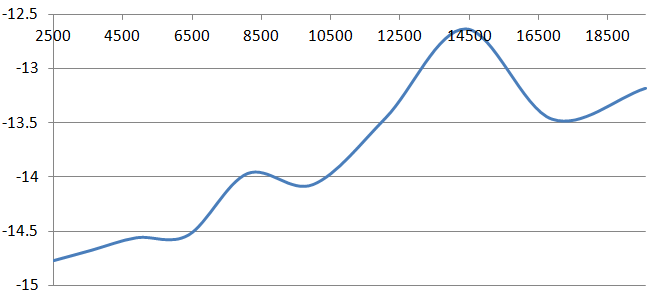
\includegraphics[width=.6\textwidth]{img/test/matrix}
    \caption{Логарифм ошибки при тестировании реализации метода матричной 
    прогонки}
    \label{fig:testMatrix}
\end{figure}

\subsubsection{Тестирование алгоритма построения интерполяций}
При тестировании построения интерполяций проверялись следующие параметры 
полученных функций: во-первых, в узлах задающей таблицы интерполированное 
значение должно совпадать с данным; во-вторых, между узлами таблицы 
интерполированные значения должны совпадать с ожидаемыми от используемого 
интерполятора -- т.е. средние значения для линейного интерполятора, экспоненты 
среднего логарифма для экспоненциального интерполятора и т.д.

Тесты совпадения значений в узлах проводились для таблиц мерностей от 1 до 3. 
Тесты корректности работы интерполяторов проводились на одномерных таблицах.

\subsubsection{Тестирование сериализации данных}
Корректность сериализации данных проверялась для следующих видов данных:
\begin{itemize}
    \item RegularGrid
    \item IrregularGrid
    \item PolarField
\end{itemize}

Также проверялась сериализация и десериализация многомерных таблиц для 
измерений от 1 до 3.

\subsection{Пользовательский интерфейс}
\subsubsection{Редактирование полей}
Для задания начальных приближений часто необходимо ручное редактирование полей 
скалярных величин. Для удобства этого процесса реализована утилита 
PDEFieldCreator, предоставляющая графический интерфейс для обеспечения 
возможности лёгкого редактирования начальных приближений. Внешний вид утилиты 
PDEFieldCreator показан на рисунке~\ref{fig:scrFC}.

\begin{figure}
    \centering
    \begin{minipage}[b]{.45\textwidth}
        \centering
        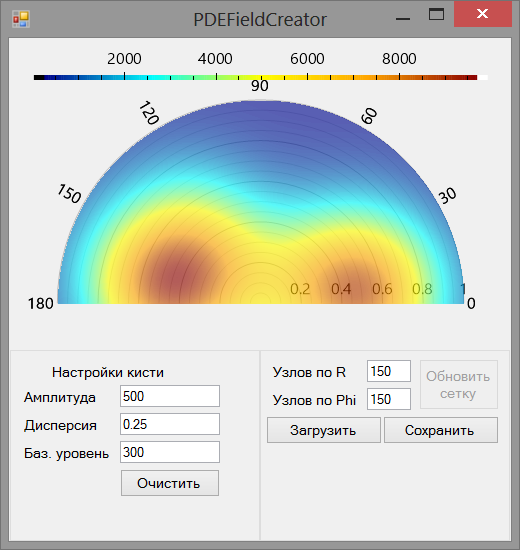
\includegraphics[width=.95\linewidth]{img/scr/fieldCreator}
        \caption{Утилита для редактирования полей}
        \label{fig:scrFC}
    \end{minipage}%
    \hspace{.1\linewidth}%
    \begin{minipage}[b]{.45\textwidth}
        \centering
        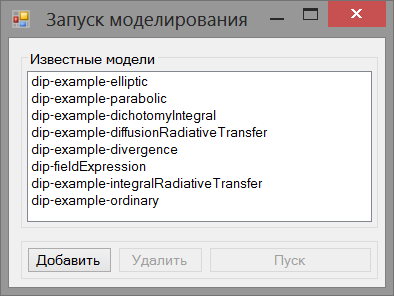
\includegraphics[width=.95\linewidth]{img/scr/launcher}
        \caption{Утилита для запуска моделирования}
        \label{fig:scrLauncher}
    \end{minipage}
\end{figure}

\subsubsection{Исполнение модели}
Утилита PDESS не имеет графического интерфейса и предназначена для работы из 
командной строки. Для повышения удобства пользования была так же создана 
утилита PDESS-GUI, предоставляющая оконный интерфейс для запуска отдельных 
экспериментов. Внешний вид утилиты PDESS-GUI представлен на 
рисунке~\ref{fig:scrLauncher}.

\subsubsection{Визуализация результатов моделирования}
Для визуализации результатов моделирования была реализована утилита PDESSVis, 
позволяющая просматривать зависящие от времени результаты вычислений как 
скалярные, так и пространственные. Внешний вид утилиты для просмотра 
результатов вычислений предоставлен на рисунке~\ref{fig:scrVis}.

\begin{figure}
    \centering
    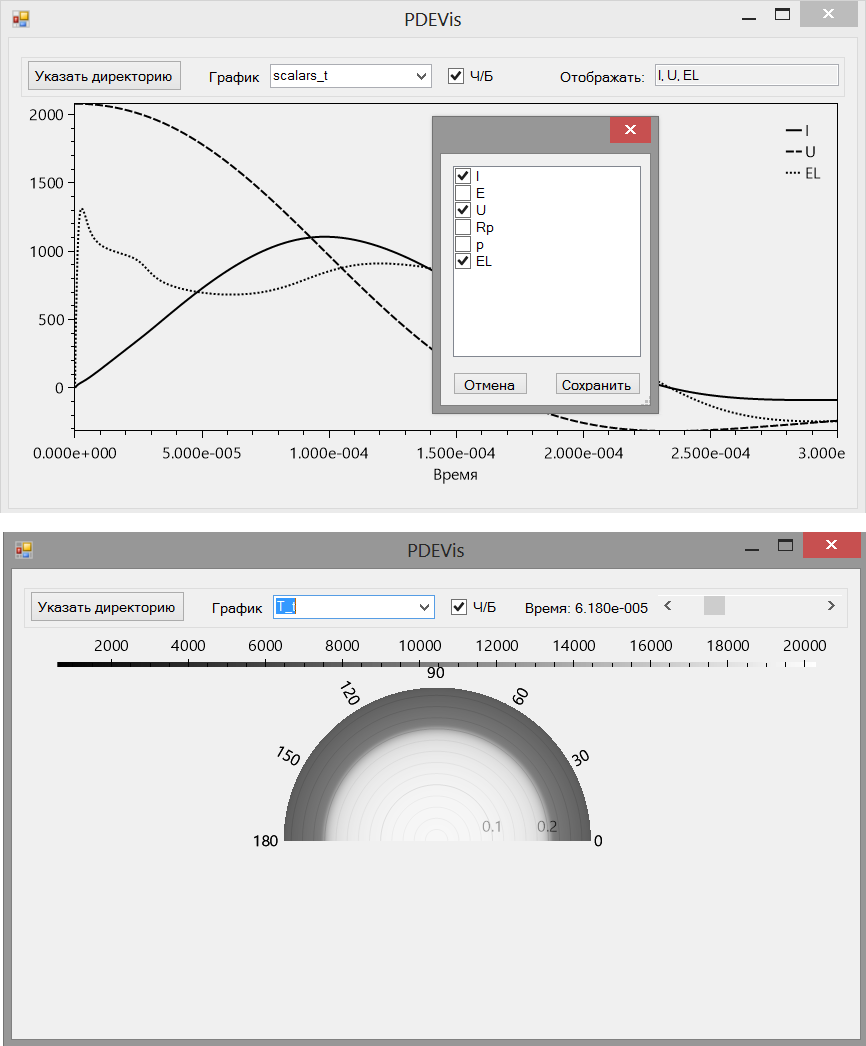
\includegraphics[width=\linewidth]{img/scr/vis}
    \caption{Просмотр результатов моделирования}
    \label{fig:scrVis}
\end{figure}

\subsection{Вывод}
Обоснован выбор языка C\# как языка программирования и приведён список 
использованных программных средств. Описаны входные и выходные форматы 
данных, описаны способы их разбора. Разработан платформо-специфичный алгоритм 
построения многомерной интерполяции, обеспечивающий достаточную скорость 
вычисления интерполированных значений, сохраняя гибкость алгоритма. Описаны 
использованные методики тестирования и приведены примеры проведённых тестов. 
Приведены изображения пользовательского интерфейса.

\section{Экспериментальный раздел}
\subsection{Введение}
В данном разделе описывается планирование вычислительных экспериментов для 
апробации разработанного программно-математического обеспечения. В качестве 
тестовых задач выбирались имеющие аналитическое решение и подходящие для 
решения выбранными методами. Приводятся результаты экспериментов и проводится 
их анализ.

\subsection{Решение эллиптического уравнения}
Для проверки решения эллиптических задач решалось уравнение~(\ref{eq:testEl}) 
стационарного теплопереноса с коэффициентом теплопроводности равным $a$. 
Получим аналитическое решение этого уравнения:
\begin{gather*}
    \frac{1}{r} \frac{\p}{\p r}(r a \frac{\p T}{\p r}) + f = 0 
    \label{eq:testEl}\\
    ra \frac{\p T}{\p r} = - \frac{fr^2}{2} + c_1\\
\end{gather*}

Введя краевое условие Неймана при $r=0: \frac{p T} {\p r} = 0$, найдём $c_1 = 
0$. Далее:
\begin{gather*}
    \p T = - \frac{f}{4 a} \p r^2\\
    T = - \frac{f r^2}{4 a} + c_2
\end{gather*}

Введя краевое условие Дирихле при $r=R: T = 0$, найдём $c_2 = \frac{5f R^2}{4 
a}$. Тогда решением~(\ref{eq:testEl}) является:
\begin{gather*}
T = \frac{f}{4 a}(R^2 - r^2)
\end{gather*}

Сравнение аналитического решения с численным представлено на 
рисунке~\ref{fig:testEl}.

\begin{figure}
    \centering
    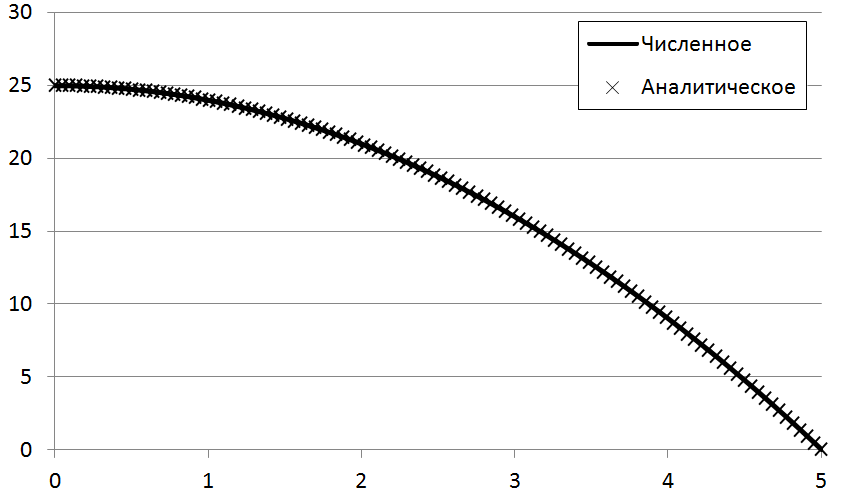
\includegraphics[width=.8\linewidth]{img/experiments/Elliptic/elVsAn}
    \caption{Аналитическое и численное решения тестовой эллиптической задачи 
    при $R=5, a=4, f=16$}
    \label{fig:testEl}
\end{figure}

Видно, что эллиптические уравнения комплекс решает точно.

\subsection{Решение параболического уравнения}
Для проверки решения эллиптических задач решалось уравнение~(\ref{eq:testPa}) 
нестационарного теплопереноса с коэффициентом теплоёмкости равным $a$ с 
предебрежимо малым коэффициентом теплопроводности. 
Получим аналитическое решение этого уравнения:
\begin{gather*}
a\frac{\p T}{\p t} = f(r)
\label{eq:testPa}\\
T(r, t) = \frac{f(r)}{a}t + c\\
\end{gather*}

Из начальных данных $T(r, 0) = 0$ находим $c = 0$, тогда 
решением~(\ref{eq:testPa}) является:
\begin{gather*}
T = \frac{f(r)}{a}t
\end{gather*}

Решение совпало с точностью до 14 знака.

\subsection{Комплексное моделирование -- эксперимент 1}\label{sec:compSlow1}
В качестве задачи комплексного моделирования была выбрана модель электрического 
разряда в комплексной плазме, описанная в~\cite{gzl,bachpaper}, . Такая модель 
содержит:
\begin{itemize}
    \item Нелинейное параболическое уравнение теплообмена
    \item Группу эллиптических уравнений переноса излучения
    \item Обыкновенные дифференциальные уравнения электрического контура
    \item Обыкновенное уравнение сохранения вещества
\end{itemize}

Диаграмма потоков данных при расчёте значений нового временного слоя такой 
модели представлена на рисунке~\ref{fig:dfdComplex}.

\begin{figure}
    \centering
    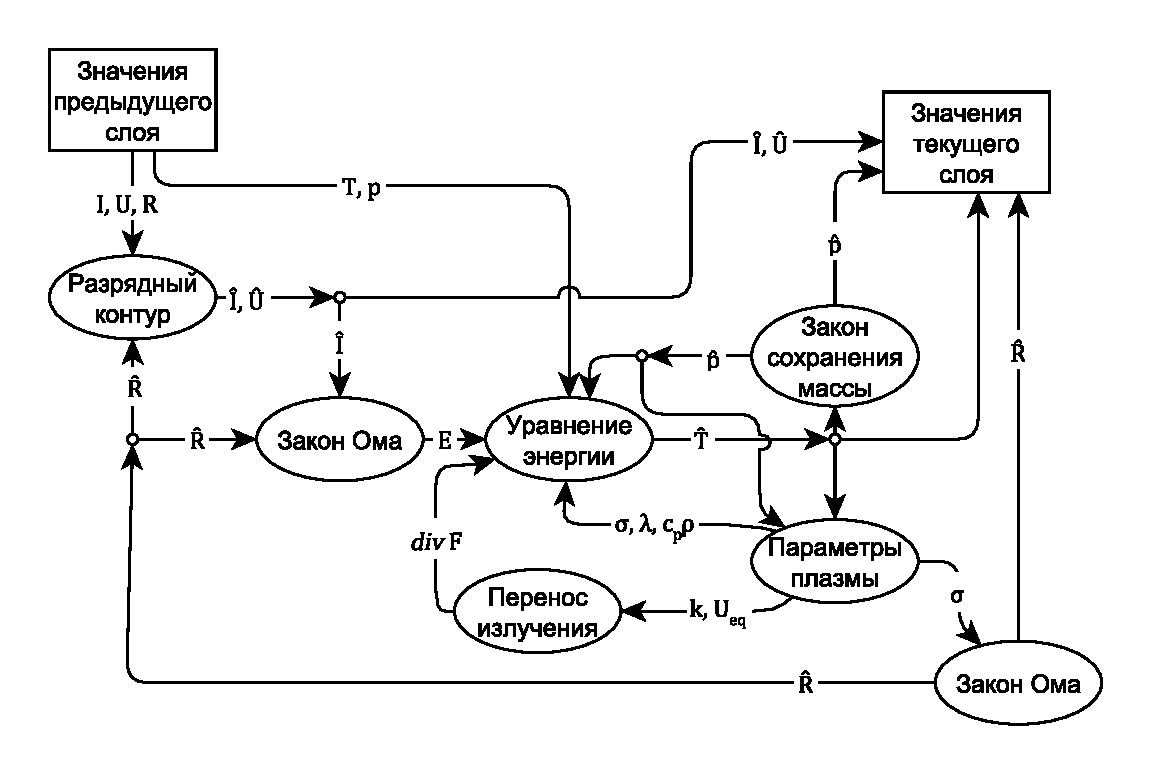
\includegraphics[width=.8\linewidth]{img/experiments/complexDiff/dfd}
    \caption{Диаграмма потоков данных при расчёте значений нового временного 
    слоя при моделировании комплексной задачи}
    \label{fig:dfdComplex}
\end{figure}

Экспериментальные данные по соответствующему эксперименту были предоставлены в 
рамках~\cite{alushtaConf}. Сравнение экспериментальных данных с рассчитанными 
значениями предоставлено на рисунке~\ref{fig:IUEComplexVsPE}.

\begin{figure}
    \centering
    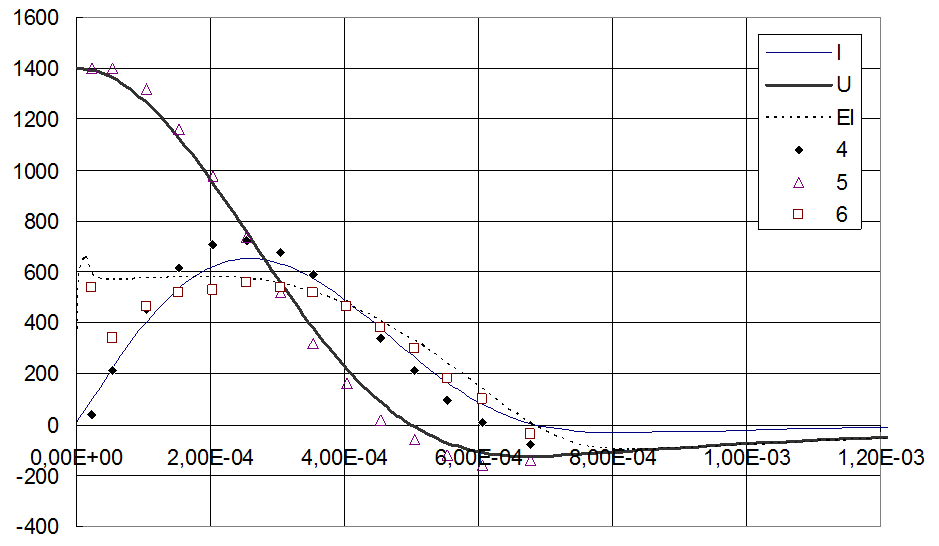
\includegraphics[width=.8\linewidth]{img/experiments/complexDiff/IUELvsPE}
    \caption{Сравнение экспериментальных данных с рассчитанными значениями, 
    эксперимент 1. 1,4 -- ток, 2,5--напряжение на конденсаторе, 3,6 -- 
    напряжение на лампе}
    \label{fig:IUEComplexVsPE}
\end{figure}

\subsection{Комплексное моделирование -- эксперимент 2}
Данный эксперимент аналогичен описанному в~\ref{sec:compSlow1}, с тем отличием, 
что перенос излучения здесь рассчитывался не в диффузионном приближении, а с 
применением описанного в~\ref{sec:intSolver} алгоритма параллельного решения 
задачи переноса излучения в интегральной постановке.

Сравнение полученных параметров контура с таковыми 
эксперимента~\ref{sec:compSlow1} предоставлено на рисунке~\ref{fig:EComplexvsC1}

\begin{figure}[h]
    \centering
    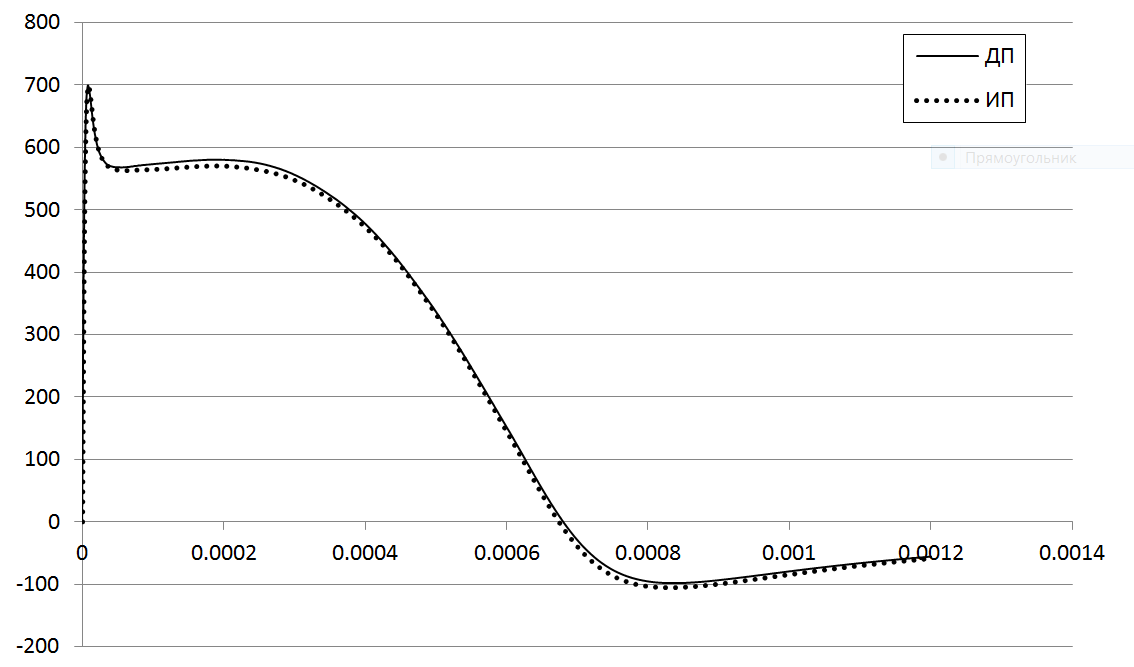
\includegraphics[width=.5\linewidth]{img/experiments/complexInt/EvsDiff}
    \caption{Сравнение рассчитанной напряжённости поля  при использовании 
    диффузионного приближения и интегральной постановки ЗПИ}
    \label{fig:EComplexvsC1}
\end{figure}

\subsection{Комплексное моделирование -- эксперимент 3}
Данный эксперимент аналогичен описанному в~\ref{sec:compSlow1}, с тем отличием, 
что начальное приближение температуры было взято не осесимметричным. Развитие 
разряда показано на рисунке~\ref{fig:comp3t}.

\begin{figure}
    \centering
    \begin{subfigure}{.5\textwidth}
        \centering
        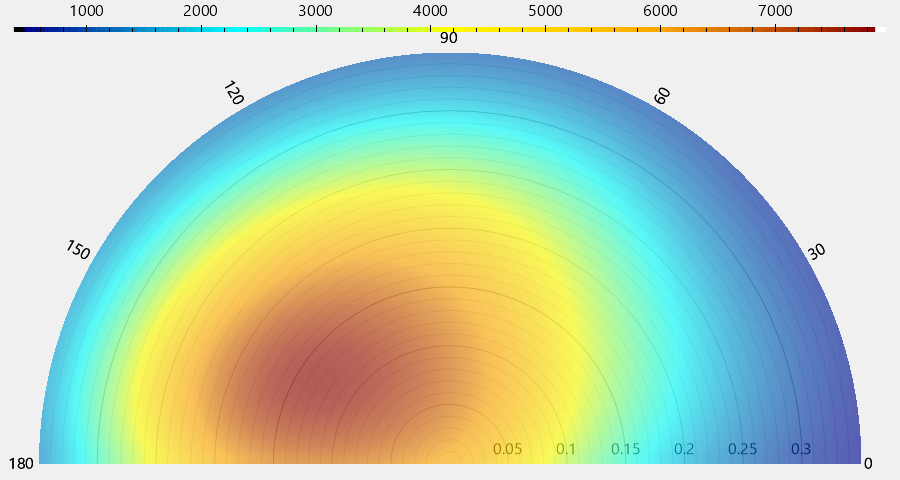
\includegraphics[width=\linewidth]{img/experiments/complexAsymm/temp-0}
        \caption{Для $t=0$мкс}
    \end{subfigure}%
    \begin{subfigure}{.5\textwidth}
        \centering
        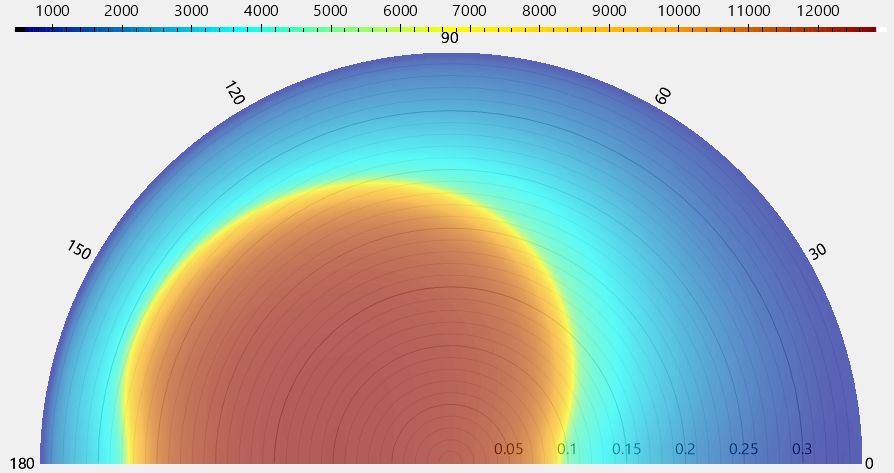
\includegraphics[width=\linewidth]{img/experiments/complexAsymm/temp-89}
        \caption{Для $t=89$мкс}
    \end{subfigure}
    
    \begin{subfigure}{.5\textwidth}
        \centering
        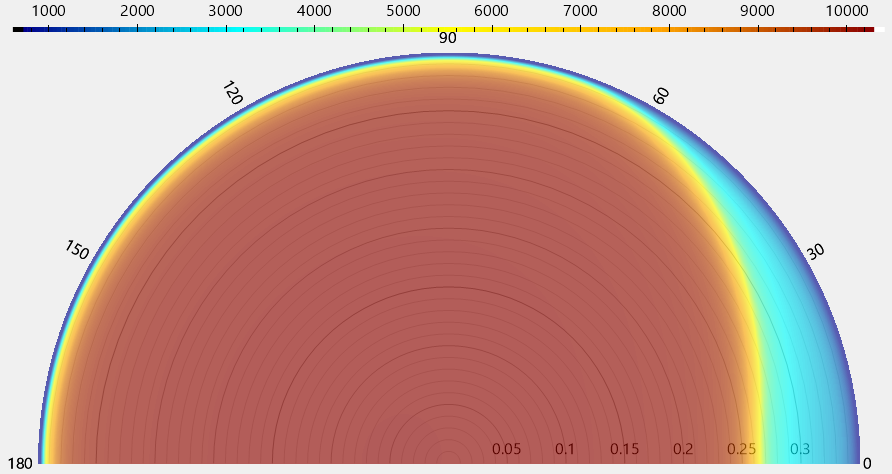
\includegraphics[width=\linewidth]{img/experiments/complexAsymm/temp-492}
        \caption{Для $t=492$мкс}
    \end{subfigure}
    \caption{Рассчитанный температурный профиль}
    \label{fig:comp3t}
\end{figure}

\subsection{Вывод}
Проведены вычислительные эксперименты и приведены результаты моделирования.
Проведено сравнение результатов решения параболических и эллиптических задач с 
их аналитическими решениями.
Сравнение с реальными экспериментальными данными показало как качественное 
(наличие мелких деталей, таких как уход в колебательный режим и провал 
напряжённости поля на стадии развития разряда), так и количественное (в 
пределах 5-10 \%) совпадение.
Результаты экспериментов позволяют утверждать о корректности разработанного ПМО 
и его применимости для независимых расчётов.

\section{Заключение}
Сформулируем основные результаты работы:
\begin{itemize}
    \item Выбраны классы уравнений, решаемые комплексом, и сформулированы 
    алгоритмы их решения
    \item Разработан метод и алгоритм расчёта в достаточной степени 
    произвольной комплексной модели
    \item Построены однородные консервативные разностные схемы для уравнений 
    модели, обеспечивающие необходимую точность вычислений
    \item Разработана и представлена с помощью диаграмм IDEF0, DFD и классов 
    структура ПО. Разработаны структуры хранения данных.
    \item Выполнена программная реализация разработанных алгоритмов, раз    
    работан пользовательский интерфейс, содержащий инструменты для формирования 
    начальных данных, моделирования и просмотра результатов эксперимента.
    \item Разработан алгоритм расчёта переноса излучения в интегральной 
    постановке, и его включением в расчёт показана расширяемость комплекса 
    дополнительными видами уравнений.
    \item Проведены эксперименты с целью апробации разработанного ПМО. 
    Выполнено качественное и количественное сравнение результатов экспериментов 
    с теоретическими и экспериментальными данными других авторов. Показано, что 
    разработанное ПО позволяет претендовать на точность порядка 7-20%.
\end{itemize}

Разработанное ПМО показало удовлетворительное совпадение результатов 
вычислительного эксперимента с результатами других вычислительных и физических 
экспериментов, что позволяет рекомендовать его для использования в научных 
исследованиях.

\section{Список литературы}
\printbibliography[heading=none]

\end{document}
